\section{Introduction}
The economic benefits of free trade are arguably one of the most uncontroversial results of economic research, both theoretically and empirically. However, to this date, free trade is by no means uncontroversial in the public sphere, as is evidenced by the fierce opposition that the proposed transatlantic free trade agreement between the US and Europe is facing. Hence, international trade has remained an active field in economic research, a field which has seen major advancements in the past two decades in incorporating firm-level heterogeneity coupled with consumer love of variety into trade models that can account for the firm-level responses to increasing trade openness and the large share of intra-industry trade in the international flow of goods and services \footnote{A comprehensive survey of trade models with love of variety preferences and firm-level heterogeneity can be found in \citet*{MelitzTrefler2012}.}. This new vintage of trade models predicts additional welfare gains from trade stemming from reallocations of production to more productive firms (as in \citealp{Melitz2003}) or increases in firms' efforts to innovate (as in \citealp{GrossmanHelpman1990}). To some extent, these new models of trade also help reconcile the unambiguously positive stance of economic researchers on trade liberalization with the public opposition to it -- models taking into account explicitly the heterogeneity across agents of firms within a country show that while on aggregate there are significant efficiency gains from free trade, there are also firms and workers who will lose out individually, and can only benefit from a trade liberalization if either the aggregate gains are redistributed in some way to ensure a Pareto improving allocation, or if they can benefit from the reallocation of production to more productive firms by switching to those firms. \citet{DixCarneiro2014} builds a structural model of the Brazilian labour market to estimate the labour market effects of trade liberalization and finds that, depending on the assumptions about capital mobility, the reallocation of workers across sectors can take up to 30 years. \\
While these new models of international trade are well grounded in empirical evidence coming from micro data, there are surprisingly few tests of the model predictions for aggregate variables which are decisive for the predicted welfare gains from trade. Recently, \citet{Arkolakisetal2012a,Arkolakisetal2012b} call into question the importance of firm-level heterogeneity by showing that in a class of trade models, the additional welfare gains are fairly small and actually even smaller if consumers don't have CES utility. The response of \citet{MelitzRedding2013} shows that there is still considerable disagreement over how to theoretically evaluate the additional welfare gains from firm selection, and \citet{CostinotRodriguez2014} review the effects of trade liberalizations in a wider class of new trade models to highlight the importance of the market structure under consideration -- depending on whether a one- or multi-sector model is used and the degree of competition assumed, gains from trade are estimated to range from 4\% to 40\% of non-free-trade welfare. These facts motivate us to test the Melitz-Ottaviano model directly in aggregate data on prices, markups and productivity. To do so, we estimate the effects of trade liberalization on the competitive environment in manufacturing markets of the member countries of the North American Free Trade Agreement (NAFTA). We employ an estimation procedure based on the \citet{MelitzOttaviano2008} model introduced by \citet{Chen2009}, which to our knowledge is the only empirical application of a model with firm-level heterogeneity on aggregate data. \citet{Chen2009} derive estimable regression equations from the model's equilibrium conditions that allow us to test the effects of trade openness on relative price levels, markups and labour productivities of two trading partners. It is further possible to differentiate between the effects of trade in the short run, which, in the model, refers to an economy without relocation decisions for firms, and in the long run, when firms are free to choose their home market for production. However, as the underlying model is static, no direct results on the time path of the impact of trade liberalization can be obtained. We try to address this issue by dividing our sample in ways that make it more amenable to a model-based estimation. Contrary to \citet{Chen2009}, we directly observe tariff rates between the three countries in our sample and hence use those as a direct measure of trade openness. Additionally, we test for the effects of third-country trade openness on the relative performance of two countries that are linked through trade, predictions for which can be derived from the multi-country version of the Melitz and Ottaviano model. Our dataset comprises of 64 manufacturing sectors in Canada, Mexico and the US, covering the time period from the introduction of the US-Canadian free trade agreement CUSFTA in 1988 up to 2010, which gives us reason to believe that we are able to capture the long run effects of policy changes even in industries with low firm churning rates. \\

Our findings support the main model predictions, with tariff barriers stifling domestic competition, leading to higher producer prices and markups as well as lower productivity. In the immediate years after the free-trade agreement when tariff barriers are reduced, relative prices and markups decrease as relative productivity increases, thus giving rise to competitive effects. The results in the long-run, however, are not as clear cut, with some effects reversing as predicted by the model while some effects persist. This is also confirmed by directly looking at the reaction of industries with different entry barriers to changes in trade openness. \\
\vspace{0.5cm} \\
The paper is organized as follows: Section \ref{sec:lit} gives a survey of the previous literature assessing the effects of trade liberalizations in general and of NAFTA specifically. Section \ref{sec:mo} briefly summarizes the Melitz and Ottaviano (2008) model, derives the most important equilibrium conditions and explains the estimation strategy used in \citet{Chen2009}. Section \ref{sec:app} then presents our application of the model by giving an overview of the data used and our estimation procedure. The results of our regressions and possible shortcomings as well as extensions of our approach are discussed in Section \ref{sec:disc4}; Section \ref{sec:conc} concludes.

\newpage

%%%%%%%%%%%%%%%%%%%%%%%%%%%%%%%%%%%%%%%%%%%%%%%%%%%%%%%%%

\section{Related Literature}\label{sec:lit}

As free trade has been an active topic in economic research since the times of Ricardo, the literature on the welfare gains from trade is immense. Of particular interest to us of course are papers that investigate the economic effects of NAFTA directly, as well as papers that form the theoretical foundation for our estimation strategy.

The effects of free trade in North America have been scrutinized in a large number of papers over the past two decades, starting with work on the predecessor to NAFTA, the 1987 Canada and US free trade agreement (CUSFTA). \citet{Head1999} document rationalization effects in Canadian plants as a reaction to decreases in Canadian import duties. \citet{Trefler2004}, focusing on the CUSFTA, uses a reduced form econometric approach to find large improvements in labour productivity and decreases in employment after the implementation of CUSFTA, coupled with slightly lower import prices and larger volumes of trade. \citet*{Fukao2003} derive regression equations from a partial equilibrium model with imperfect competition to estimate the extent to which NAFTA was trade diverting rather than creating and find responses that vary by industry. \citet{Romalis2007} examines both CUSFTA and NAFTA with a strategy based on estimating demand and supply elasticities and finds a large effect of NAFTA on trade volumes, with only minor price changes and, subsequently, only small changes in welfare. \citet{Calderon-Madrid2007} use plant-level panel data from Mexico to show that while productivity increases followed the tariff reductions, the responses of plant-level productivity are very unevenly distributed, with larger plants benefiting disproportionately from productivity increases. The \citet{Melitz2003} model that is at the heart of our analysis is also put to a test with US manufacturing data by \citet*{Bernard2006a}, who use plant-level data to estimate the effects of changes in the costs of trade, as measured by tariff rates and transportation cost, on productivity growth and firm entry and exit. Their findings confirm the micro-level implications derived from the assumptions on the productivity distribution in \citet{Melitz2003}, which we will highlight in the following section. Other papers have used the structure provided by the \citet{MelitzOttaviano2008} model to assess the effects of trade liberalization in other parts of the world: \citet{Bellone2008} use price-cost margins of French manufacturing firms to test the models predictions on the effects of market size, import penetration and exporting status on markups and productivity and confirm that all predictions hold. \citet{Corcos2011} estimate structural parameters in order to simulate counterfactual scenarios by changing the costs of trade between countries. Their exercise shows that the firm selection mechanism is crucial for the magnitude of the welfare gains from trade and the potential gains for a country depend on country size as well as remoteness. The paper that is closest to our own work is \citet{Chen2009}, who use the equilibrium expressions for prices, markups and productivity from the Melitz-Ottaviano model to estimate the effects of trade liberalization using a dataset that includes data on 10 manufacturing sectors in seven European countries for the period 1989-1999 with country-pair regressions. There results suggest that trade openness leads to an increase in competitiveness in the short-run with diminishing and at times reversed effects in the long-run, as predicted by the model. 

%%%%%%%%%%%%%%%%%%%%%%%%%%%%%%%%%%%%%%%%%%%%%%%%%%%%%%%%%

\section{Model and Estimation Equations}\label{sec:mo}

The \citet{MelitzOttaviano2008} model is a synthesis of the contributions of \citet{Melitz2003}, who introduces firm heterogeneity through random draws of a cost parameter for firms entering the market, and \citet{Ottaviano2002}, who develop a model with endogenous markups arising from a linear consumer demand system with horizontal product differentiation. The model yields equilibrium conditions that determine a cost cut-off level, i.e. a level of productivity below which firms are not able to compete in the marketplace. This cut-off level uniquely determines all relevant aggregate variables in the model, namely the distribution of prices, markups and productivity. Importantly, the equilibrium conditions of the model economy are different depending on whether firm entry is allowed or not. Without firm entry, the model captures a short-run equilibrium, with the cost cutoffs in two markets given by:
\begin{align}
N = \bar{N} \left( \frac{c_D}{c_M} \right)^k + \bar{N}^* \frac{1}{\tau^k}\left( \frac{c_D}{c_M^*} \right)^k \label{eq:m-o-supply-n} \\
N^* = \bar{N}^* \left( \frac{c_D^*}{c_M^*} \right)^k + \bar{N} \frac{1}{\left( \tau^* \right)^k}\left( \frac{c_D^*}{c_M} \right)^k \label{eq:m-o-supply-n*}
\end{align}
Here, a star denotes the foreign market, $\bar{N}$ is the fixed number of incumbents in a market and $N$ is the number of firms that are producing. $c_M$ is the upper bound of the distribution of cost draws, $c_D$ is the cut-off level, i.e. the highest cost draw that allows a firm to earn non-negative profits. $\tau>1$ is the iceberg cost of trade faced by foreign companies exporting to the domestic market and can be interpreted as a measure of trade costs, tariffs and other impediments to trade. \\
The long-run equilibrium of the economy allows for firm entry into a market, so that the number of firms in a market is now endogenously determined by a zero profit condition for entrants that balances a fixed cost of entry with the expected profits when drawing a cost level from the (known) cost distribution of a country. The equilibrium conditions pinning down the cost cut-off are
\begin{align}
c_D = \left[ \frac{\phi c_M^k}{L} \frac{1-(\tau^*)^{-k}}{1-(\tau\tau^{*})^{-k}} \right]^{\frac{1}{k+2}} \\
c_D^* = \left[ \frac{\phi c_M^k}{L^*} \frac{1-\tau^{-k}}{1-(\tau\tau^{*})^{-k}} \right]^{\frac{1}{k+2}},
\end{align}
where $L$ is the size of the domestic market. Since all aggregate variables in the Melitz and Ottaviano model are linear functions of the cost cut-off, equations describing the relative price, markup and productivity levels in two countries connected by trade can easily be found by simply dividing the expressions for $c_D$ by those for $c_D^*$. This gives, for the price level in the short run:
\begin{align}
\left( \frac{\bar{p}}{\bar{p}^*} \right)^k = \left( \frac{c_D}{c_D^*} \right)^k = \left(\frac{c_M}{c_M^*} \right)^k \frac{\bar{N}^*}{\bar{N}} \frac{N}{N^*} \frac{1 + \frac{\bar{N}}{\bar{N}^*} \frac{1}{(\tau^*)^k} \left( \frac{c_M^*}{c_M} \right)^k}{1 + \frac{\bar{N}^*}{\bar{N}} \frac{1}{\tau^k} \left( \frac{c_M}{c_M^*} \right)^k} \label{eq:mo-relprice-sr}
\end{align}
and in the long run: 
\begin{align}
\left( \frac{\bar{p}}{\bar{p}^*} \right)^{(k+2)} = \left( \frac{c_D}{c_D^*} \right)^{(k+2)} = \left( \frac{c_M}{c_M^*} \right)^k \frac{L^*}{L} \frac{1-\frac{1}{\tau^k}}{1 - \frac{1}{(\tau^*)^k}} \label{eq:mo-relprice-lr}
\end{align}
These two equations capture one of the central predictions of the Melitz and Ottaviano model: asymmetrical trade liberalizations will have opposing effects on competitiveness in the short and the long run. By equation (\ref{eq:mo-relprice-sr}), lowering trade barriers induces a fall in the cost cutoff, and hence decreases in prices and markups and increases in productivity. In the long run, however, the effects are reversed, as an increase in trade costs induces firms to choose the relatively more protected market for production, thereby increasing competition in markets that are shielded from foreign firms. \\
\citet{Chen2009} show that it is possible to substitute out the trade cost term with an openness term that is derived from a measure of foreign firms market share in the domestic market. However, since we are interested in the effect of tariff rates on competitiveness, we use tariff data directly as a proxy for $\tau$. This strategy should pick up the effects of tariff rates in our estimation if other determinants of trade openness (e.g. oil prices \citep{Kilian2009}, credit conditions \citep{Chor2012}, shared culture and language between countries) do not vary systematically across industries. However, as a first step, we will replicate their analysis exactly in our data set (albeit with different instruments for openness), which requires us to make the same substitution, which is:
\begin{equation}
\frac{1}{\tau^k} \left( \frac{c_M}{c_M^*} \right)^k = \frac{\theta}{1-\theta} 
\end{equation}

Similarly, an expression for the average markup can be derived. The determination of the average markup is equivalent to the one for average prices so expressions for the short-- and long--run impacts of openness on markups can readily be derived. Somewhat more problematic is the index for productivity, as the model requires knowledge of a firm's unit costs $c$, which are not observable. Chen et al. work around this issue by assuming away differences in capital costs, so that average industry productivity can be approximated by the ratio of nominal wages to labour productivity: $\bar{c} = \frac{w}{z}$. If it is additionally assumed that unit labour costs only depend on nominal wages, the ratio of domestic to foreign labour productivity can be written as:
\begin{equation}\label{eq:chen-lab-prod}
\frac{z}{z^*} = \frac{w}{w^*} \frac{\bar{c}^*}{\bar{c}}
\end{equation}
If the least competitive firm in an industry with a productivity draw at the upper bound of the distribution $c_M$ has labour productivity $z_M$ and labour is perfectly mobile between firms, equation (\ref{eq:chen-lab-prod}) implies $\frac{z}{z^*} = \frac{w}{w^*} \frac{c_M^*}{c_M}$. This relationship can then be used in an analogous fashion as before to construct an expression relating openness to productivity. In the short run, equation (\ref{eq:chen-lab-prod}) can be amended to yield:
\begin{equation}\label{eq:chen-prod-sr}
\left( \frac{z}{z^*} \right)^k = \left( \frac{z_M}{z_M^*} \right)^k \frac{(\bar{N}/N)}{(\bar{N}^*/N^*)} \frac{1+ \frac{\bar{N}*}{\bar{N}} \frac{\theta}{1-\theta}}{1+ \frac{\bar{N}}{\bar{N}^*} \frac{\theta^*}{1-\theta^*}} 
\end{equation}
Higher values of $\theta$ thus lead to higher productivity (conditional on $\bar{N}/N$), as they force lower productivity firms to shut down production. For the long run, equation (\ref{eq:mo-relprice-sr}) combined with the expression for labour productivity gives:
\begin{equation}\label{eq:chen-prod-lr}
\left( \frac{z}{z*} \right)^{k+2} = \left( \frac{w}{w^*} \right)^2 \frac{L}{L^*} \left( \frac{z_M}{z_M^*} \right)^k \frac{1-\frac{\theta}{1-\theta}}{1-\frac{\theta^*}{1-\theta^*}}
\end{equation} 
Larger markets exhibit higher labour productivity, while the effects of $\theta$ and $\theta^*$ are the opposite of those in the short--run.

%%%%%%%%%%%%%%%%%%%%%%%%%%%%%%%%%%%%%%%%%%%%%%%%%%%%%%%%%

\subsection{The Role of Market Entry}
Following the arguments in \citet{Trefler2004}, we want to exploit the nature of NAFTA being close to a natural experiment and hence try to identify the effect of the policy measures (i.e. the changes in tariff rates) separately from the effects of trade openness in general. There is evidence that trade openness -- measured by the import penetration of a certain country or industry, as in \citet{Chen2009} -- is affected by a number of external forces, including oil prices \citep{Kilian2009}, credit conditions \citep{Chor2012}, shared culture and language between countries and many more. Therefore, we deconstruct the iceberg costs of trade into two parts: $\tau^{lh}=\frac{Tr^{lh}}{\theta^{lh}}$, where $Tr^{lh}>1$ is the tariff rate for trade between countries $l$ and $h$ and $\theta^{lh}>1$ captures the additional costs of trade imposed by the aforementioned factors. Then, the import penetration can be viewed as a measure of $\theta^{lh}$, as in Chen et al. (2009), while a carefully constructed tariff measure can directly account for the effect of NAFTA-mandated changes in the trade environment. Obviously, the import penetration in a sector depends on the tariff measure as well, so an instrumental variable approach has to be taken in order to identify this effect. We defer the discussion of the construction of the tariff measure and the choice of instruments to the following chapter. Prior work of \citet{Bernard2006} suggests that tariff rates throughout the 1980s, at an average level between four and five percent, accounted for about the same fraction of trade costs as costs directly attached to shipping the good, i.e. freight and insurance, so we expect them to have a sizeable impact on trade flows between countries and hence the competitive environment. \vspace{0.5cm} \\

As we have seen in the exposition of the Melitz and Ottaviano model above, there is one crucial caveat in taking the model to the data: due to the static nature of the model, the comparative static results just compare one steady state with another, while being silent about the transitional dynamics. The estimation strategy of \citet{Chen2009} tries to account for this by estimating an error correction model to identify the long-run separately from the short-run, but their results -- just as ours -- are mixed for the long run and it cannot be ruled out that this is due to the estimation procedure. Therefore, we try to address this issue in a more direct way: as short- and long-run in the model differ only in the possibility of firm entry, we separate industries into those with a fixed number of firms and those with low entry barriers. This distinction then gives us industries that represent the short- and long-run and we can directly investigate whether the coefficients on the relevant variables differ significantly\footnote{We were inspired to do so by \citet{Head1999} who use the classification to test competing theories of trade that rely on different market structures.}. This approach, however, leads to two issues that need to be addressed before implementation. First, it is not \textit{a priori} obvious how to measure the entry conditions in an industry; while the theoretical model uses the number of firms, this could in practice either refer to firms or to establishments (i.e. different production sites run by the same parent company), or even to employees, as firms in the model use unit labour input. Second, there is no reason to believe that different measures of entry and exit dynamics are exogenous with respect to trade openness -- indeed in the model trade openness is a key factor in the entry decision of firms, but in the real world there might be various other factors that might lead to industries being asymmetrically affected by a change in trade costs, hence biasing our results. To tackle both these issues, we aim to construct a robust measure of industry dynamics by aggregating multiple studies that examine firm and employment turnover in Canada, Mexico and the United States as well as Europe over different time periods. With this, we hope to identify those industries that are either very dynamic or very static over a broad set of different measures, regions and time periods. Table \ref{tb:market_lit} gives an overview of the studies used and a glance at their respective results, showing considerable variation in the dynamics of entry and job creation in different manufacturing sectors.
 
\begin{center}
\begin{table}
\begin{tabular}{|p{2.8cm}|p{4cm}|p{4cm}|p{4cm}|}
\hline
\textbf{Study}  &  \textbf{Subject}  &  \textbf{Highest Turnover}  & \textbf{Lowest Turnover} \\
\hline 
\hline
\citet{Dunne1988} & Entry Rates (4-yearly) \newline U.S. \newline 63-82    & Instruments (60.3) \newline Lumber (49.70) \newline Printing (49.0)  & Leather (29.4) \newline  Food Processing (23.9) \newline Tobacco (20.5) \\  
\hline
Samianego (2008)   & Entry Rates (yearly)  \newline Europe \newline 97-04  & Paper, printing, software (15.6) \newline Textiles (11.9) \newline Petroleum and Coal (11.9) & Chemicals (9.5) \newline Plastics (9.4) \newline Food Products (9.1) \\
\hline 
\citet{Brown2004}  & Employment renewal    \newline Canada \newline 73-96  & Plastic (79.5) \newline Furniture (79.4) \newline Fabricated Metals (77.2) & Primary Metals (33.6) \newline Paper (32.4) \newline Tobacco (4.2) \\
\hline
\citet{Foster2006} & Job creation (yearly) \newline U.S. \newline 72-98     & Lumber (11.8) \newline Apparel (11.2) \newline Miscellaneous (11.0) & Paper (5.9) \newline Petroleum (5.9) \newline Tobacco (5.1) \\
\hline
\citet{Baldwin1994} & Job turnover (yearly) \newline Canada \newline 73-86 & Furniture (26.5) \newline Machinery (26.3) \newline Lumber (25.7) & Petroleum (14.1) \newline Primary Metals (13.5) \newline Paper (10.7)  \\
\hline
\citet{Baldwin1994} & Job turnover (yearly) \newline U.S. \newline 73-86 & Lumber (27.2) \newline Apparel (25.5) \newline Leather (22.5) & Petroleum (14.6) \newline Chemicals (14.0) \newline Paper (13.3) \\
\hline   
\end{tabular}\caption{Market Structure measures used, numbers in percent}\label{tb:market_lit}
\end{table} 
\end{center}

In order to aggregate the different studies, we compute percentile-based rankings of the industries for each study (to account for the different number of industries across studies) and then average the percentiles across studies. Based on these average percentiles, we can then split the sample according to the short- and long-run distinction made in the model: those industries above the 70th percentile are taken to represent the dynamic, "free entry" sample and thus the long run, while those industries below the 40th percentile are taken to represent the short run. This procedure leads us to split the sample three-ways: Tobacco, Food Processing, Paper, Chemicals, Primary Metals and Petroleum industries fall into the long run category, while Furniture, Wood, Non-electrical Machineries, Fabricated Metals, Printing, Apparel, and Instruments are taken to represent the short run of the model. The remaining industries are too close to the median to be classified either way and are thus dropped from the sample, which leaves us with 1863 year-industry-country pair observations for the free entry sample, and 1701 observations for the fixed entry sample\footnote{Due to different classification systems, the aggregation of studies was not always exact and some industry groups are quite heterogeneous when sub-industries are considered. For further details on the aggregation see Appendix B}. \\
A little thought experiment may clarify the role that market entry effects play in muddling the distinction between short-- and long--run equilibria. The Melitz and Ottaviano (2008) model yields opposing predictions on the effects of trade liberalization on country-level economic variables such as prices, productivity and mark-ups. The reason for the differences, as we have seen, lies in the assumptions on market structure: there are two different equilibria depending on whether entry into a market is allowed. We repeat them here for convenience:
\begin{align*}
c_D^k &= c_M^k \frac{\bar{N}^*}{N^*} \left( 1+ \frac{\bar{N}}{\bar{N}^*} \frac{\theta^*}{1-\theta^*} \right) \\
c_D^{k+2} &= \frac{\phi c_M^k}{\Upsilon L} \left(1- \frac{\theta^*}{1-\theta^*} \right)
\end{align*}
In model terms, only one of these two equations holds at any given time, and it is posited that the first equation captures the short run effects of trade liberalization, while in the long run firms are allowed to enter the markets and the effects of trade barriers are determined by the second equation. No further assumptions on the nature of the firm's entry decisions or capital adjustment costs are made that could help separate short- from long run. However, in reality, it seems to be more natural to assume that there is a gradual evolution from one equilibrium to the other, and this view is borne out by data on firm entry and exits showing that in a given year, only between five and ten percent of firms in a given industry are new entrants, while over longer horizons this figure goes up to 80 percent. Hence, it seems to be reasonable to model the transition from the short- to the long run equilibrium by introducing a parameter $\alpha$ that governs the fraction of firms entering an industry. The effects of this parameter are most clear on the productivity side, given that firms cannot change their productivity level, the new productivity distribution will be a weighted average of new entrants' and existing firms' productivity. As the examples in Chen et al. are formulated with respect to relative prices, and we are using their notation, we will discuss the effects of limited firm entry in the price level case as well. The argument carries through if one is ready to assume a nominal rigidity that prevents incumbents from re-optimizing their prices, similar to the assumptions made in New Keynesian monetary models. Similar to the productivity level, the price level is then a weighted average of new and old prices (for simplicity, here we abstract from substitution effects induced by the new relative prices of new and old producers):
\begin{align*}
\bar{p} &=\alpha \bar{p}^{LR} + (1-\alpha) \bar{p}^{SR} \\
				&=\alpha c_D^{LR} + (1-\alpha) c_D^{SR} \\
        &=\alpha \left( \frac{\phi c_M^k}{\Upsilon L} \left(1- \frac{\theta^*}{1-\theta^*}  \right) \right)^{\frac{1}{k+2}} + (1-\alpha) \left(c_M^k \frac{1}{ \frac{\bar{N}}{N}\left( 1+ \frac{\bar{N}^*}{\bar{N}} \frac{\theta}{1-\theta} \right) } \right)^{\frac{1}{k}}							
\end{align*}
where the second line drops the constant linking price level and cost cut-off for notational simplicity. It can easily be seen that the introduction of the $\alpha$ parameter makes the expression for the price level hugely complicated and eliminates the possibility to cancel out most constant terms by using relative prices as was done in \citet{Chen2009}. Obviously, the above expression is impossible to take to the data in the hope of identifying any of the parameters. \\
Let's consider a simplified version of the above. Assume that relative prices levels in the short- and long run, respectively, are given by:
\begin{align*}
\frac{\bar{p}^{SR}}{\bar{p}^{*SR}} = \left( \frac{c_M}{c_M^*} \right)^k \frac{(\bar{N}^* / N^*)}{(\bar{N} / N)} \frac{\rho^*}{\rho} \\
\frac{\bar{p}^{LR}}{\bar{p}^{*LR}} = \left( \frac{c_M}{c_M^*} \right)^k \frac{L^*}{L} \frac{(1-\rho^*)}{(1-\rho)}
\end{align*}
This is a simplified version of the equilibrium conditions in Chen et al. using the notation of Melitz and Ottaviano in which trade freeness is measured by $\rho \in (0,1)$. It captures the main essence of the model, in the short run relative prices depend on the number of firms and negatively on trade freeness (increasing $\rho$ will decrease $\bar{p}$), while in the long country size matters and prices depend positively on trade freeness (increasing $\rho$ decreases $1-\rho$ and thus increases $\bar{p}$). Now assume further, that price setting decisions and substitution behaviour of consumer is such that we can aggregate \textit{relative} price levels in the same way we aggregated individual price levels before. Then:
\begin{align*}
\frac{\bar{p}}{\bar{p}^*} &= \alpha \frac{\bar{p}^{LR}}{\bar{p}^{*LR}} + (1-\alpha) \frac{\bar{p}^{SR}}{\bar{p}^{*SR}} \\
													&= \alpha \left( \left( \frac{c_M}{c_M^*} \right)^k \frac{L^*}{L} \frac{(1-\rho^*)}{(1-\rho)} \right) + (1-\alpha) \left( \left( \frac{c_M}{c_M^*} \right)^k \frac{(\bar{N}^* / N^*)}{(\bar{N} / N)} \frac{\rho^*}{\rho} \right)
\end{align*}
Here, the fundamental identification problem becomes apparent: in the first term on the right hand side of the equation, the effect of $\rho$ on $\bar{p}$ is positive, while in the second term it is negative. However, the size and sign of the composite effect will be governed by $\alpha$, which is unobservable. In order to estimate the effects of trade openness on prices, we have to control for firms entry behaviour. While this might well be endogenous to changes in trade policy, it is reasonable to assume that different industries have different entry conditions due to fixed costs inherent in the business model. We can try to exploit this variation in entry conditions by sorting businesses according to the ease of entry; then, ceteris paribus, an industry with lower barriers to entry should exhibit a response to trade liberalization along the lines that the model predicts for the long run equilibrium (as the value of $\alpha$ increases, $\bar{p}$ approaches $\bar{p}^{LR}$), while an industry with high entry barriers subject to the same trade liberalization should see a very different reaction. \\
One way to alleviate this problem is by trying to use information on $\alpha$ in the estimation. Splitting the sample based on our aggregated turnover measures can be seen as a crude approximation to this, as can be the construction of dummy variables for high and low turnover industries. The most direct way, however, would be to use information on industry turnover rates directly. Obviously, this brings back the very same endogeneity problems we described above that were one reason to aggregate the studies in the first place, which makes it important to instrument for entry and exit rates in industries using turnover measurements for different periods than the one considered in the estimation. The variable construction will be explained in more detail in the next section.

\section{Application}\label{sec:app}
Starting from the equations for prices, productivity and markups derived within the Melitz-Ottaviano framework, we can derive estimable log-linearised equations analogous to those in Chen et al. The estimation equation for prices is given by:
\begin{align}
\begin{split}\label{eq:gw-estimation-prices}
\Delta \ln \left( \frac{\bar{p}_{it}}{\bar{p}_{it}^*} \right) = &\beta_0 + \beta_1 \Delta \ln \tau_{it} + \beta_2 \Delta \ln \tau_{it}^* + \beta_3 \Delta \ln D_{it} + \beta_4 \Delta \ln D_{it}^* \\ &+ \gamma \left[ \ln \left( \frac{\bar{p}_{it-1}}{\bar{p}_{it-1}^*} \right) + \delta_0 + \delta_1 \ln L_{t-1} + \delta_2\ln L_{t-1}^* + \delta_3 \ln  \tau_{i,t-1} + \delta_4 \ln  \tau_{i,t-1}^* \right] + \varepsilon_{ijt} 
\end{split}\end{align}
In the above equation, the number of firms serving the domestic market, $N$, has been replaced by the more readily observable number of domestic firms producing for the domestic market, $D$, where $D=N \left( \frac{c_D}{c_M} \right)^k$. The short--run dynamics are estimated in the first part of the equation, with regressors expressed in first differences. The long run is represented by the term in brackets. From the perspective of this model, we would expect $\beta_1>0$, an increase in domestic import tariffs increases relative prices in the short-run, and correspondingly $\beta_2>0$. The model predicts a dampening effect of the number of domestic firms on domestic prices, which should be reflected by $\beta_3<0$, and the opposite for foreign firms, $\beta_4<0$. As we expect the coefficient on the error correction term, $\gamma$, to be negative, a reversal the 

As previously discussed, all aggregate variables (prices, markups, productivity) are ultimately functions of the cost-cutoff level $c_D$, leading to very similar estimation equations for our three dependent variables. The equation markups is:
\begin{align}
\begin{split}\label{eq:gw-estimation-markup}
\Delta \ln \left( \frac{\bar{\mu}_{it}}{\bar{\mu}_{it}^*} \right) = &\beta_0 + \beta_1 \Delta \tau_{it} + \beta_2 \Delta \tau_{it}^* + \beta_3 \Delta \ln \theta_{it} + \beta_4 \Delta \ln \theta_{it}^* + \beta_5 \Delta \ln D_{it} + \beta_6 \Delta \ln D_{it}^*\\ 
&+ \gamma \left[ \ln \left( \frac{\bar{\mu}_{it-1}}{\bar{\mu}_{it-1}^*} \right) + \delta_0 + \delta_1 \ln L_{t-1} + \delta_2\ln L_{t-1}^* + \delta_3  \tau_{i,t-1} + \delta_4  \tau_{i,t-1}^* \right] + \varepsilon_{ijt} 
\end{split}
\end{align}
The effect of tariffs, openness, number of firms and market size on productivity is estimated by:
\begin{align}
\begin{split}\label{eq:gw-estimation-productivity}
\Delta \ln \left( \frac{\bar{z}_{it}}{\bar{z}_{it}^*} \right) =&\beta_0 + \beta_1 \Delta \tau_{it} + \beta_2 \Delta \tau_{it}^*  + \beta_3 \Delta \ln D_{it} + \beta_4 \Delta \ln D_{it}^*\\
&+ \gamma \left[ \ln \left( \frac{z_{it-1}}{z_{it-1}^*} \right) + \delta_0 + \delta_1 \ln L_{t-1} + \delta_2\ln L_{t-1}^* + \delta_3  \tau_{i,t-1} + \delta_4  \tau_{i,t-1}^*  \right. \\ 
&+ \left. \delta_5 \ln w_{i,t-1} +  \delta_6 \ln w_{i,t-1}^* \bigg] \right. + \varepsilon_{ijt} 
\end{split}
\end{align}
where $\delta_7$ and $\delta_8$ capture the effects of changes in nominal wages in the long run. The intercepts $\beta_0$ are introduced to capture differences in country--specific technology as Chen et al. depart from the baseline Melitz-Ottaviano model by allowing for such differences. While in the baseline, these vary by country-pair, we check the robustness of the specification by allowing fixed effects at a sectoral level. 

\subsection{Preferential Trade Liberalization}
The model results and estimation equations presented so far all referred to a 
unilateral trade liberalization in a simplified two-country setup\footnote{Note
 that a bilateral trade liberalization -- changing $\tau$ and
 $\tau^*$ by the same amount -- would not lead to the discussed short- and long 
run changes in cost cutoffs for two countries, but instead to a decline in the cost cutoffs in both countries both in the short and the 
long run.}. While making the exposition clearer and helping to elicit the effects at work in the model, this setup is clearly not an accurate description of the reality of trade relationships in modern industrialized economies. Taking the United States as an example, while the two other countries in our data set, Canada and Mexico, are its largest 
trading partners, they only account for 16.6 and 13.5\% of all US trade by value, 
respectively\footnote{See \href{http://goo.gl/2C0saQ}{Top U.S. Trade Partners, U.S. International Trade Administration}}. 
Even the largest 30 US trading partners only account for about 86\% of US trade, highlighting the fragmented nature of international trade. While the Melitz-Ottaviano model can be extended to an arbitrary number of countries, it is clearly not feasible to assemble a data set on all trade partners of the NAFTA countries. We do however want to recognize the multi-country structure of NAFTA by taking into account third country effects of trade barriers. Here, NAFTA can be interpreted as a preferential liberalization of Mexico \textit{vis-a-vis} the US and Canada, as Mexico had the highest tariff barriers to start off with. In the three country case, we expect the country with the lowest sum of bilateral trade barriers to have the lowest cost cutoff, as it becomes the best export hub. To account for this, we amend equations \ref{eq:gw-estimation-prices}, \ref{eq:gw-estimation-markup} and \ref{eq:gw-estimation-productivity} by including the relevant third country tariffs. The estimation equation for the effects of trade barriers on prices then becomes:

\begin{align}
\begin{split}\label{eq:gw-estimation-prices-third-country}
\Delta \ln \left( \frac{\bar{p}_{it}}{\bar{p}_{it}^*} \right) = 
&\beta_0 + \beta_1 \Delta \ln \tau_{it} + \beta_2 \Delta \ln \tau_{it}^* + \beta_3 \Delta \ln \tau_{it}^{ht} 
+ \beta_4 \Delta \ln \tau_{it}^{th} + \beta_5 \Delta \ln \tau_{it}^{ft} + \beta_6 \Delta \ln \tau_{it}^{th} \\ 
&+ \beta_7 \Delta \ln D_{it} + \beta_8 \Delta \ln D_{it}^* + \beta_9 \Delta \ln D_{it}^t \\ 
&+ \gamma \left[ \ln \left( \frac{\bar{p}_{it-1}}{\bar{p}_{it-1}^*} \right) + \delta_0 + \delta_1 \ln L_{t-1} + \delta_2\ln L_{t-1}^* 
 + \delta_3 \ln L_{t-1}^t+ \delta_4 \ln \tau_{i,t-1} \right. \\ 
&+ \left. \delta_5 \ln  \tau_{i,t-1}^*  + \delta_6 \Delta \ln \tau_{it}^{ht} + \delta_7 \Delta \ln \tau_{it}^{th} 
 + \delta_8 \Delta \ln \tau_{it}^{ft} + \delta_9 \Delta \ln \tau_{it}^{th} \bigg] \right. + \varepsilon_{ijt} 
\end{split}\end{align}
where now $h$ is the domestic economy, $f$ is the foreign economy, and, with a slight abuse of notation, a $t$ superscript denotes the third country for each country pair (e.g. when estimating the Canada-US relationship, $\tau^{th}$ are Mexican tariffs on Canadian goods, while $\tau^{ht}$ are Canadian tariffs on Mexican goods). Both the equations for markups and productivity will be amended accordingly. 

\subsection{Dataset}

The database we utilize covers the period 1988-2014 for NAFTA member countries -- Canada, Mexico, and the US -- and nine manufacturing sectors at the ISIC two digit level, which includes 86 industries . For our factory gate price data, we use the producer price index (PPI) as reported by CANSIM, the Banco de Mexico, and the U.S. Bureau of Labor Statistics, respectively. All indices are normalized to equal 100 in 2003. While the majority of the manufacturing data collected is reported at the two-digit level according to ISIC Rev. 3, we aggregate all data according to NACIS in order to keep consistency throughout the analysis (see Table \ref{tab:naics4diglist} for the manufacturing classification breakdown). While the main part of our analysis rests on data aggregated at the two-digit level, we were also able to assemble a data set at the four-digit level, which we will use to check the robustness of our results. 

The value of markups is not easily observable, and thus we follow the calculation as outlined in the recent literature on industrial organization, and similarly used by \citet{Chen2009}, although with a subtle modification. We compute average markups as the ratio of sectoral turnover relative to total variable costs, which are computed as the sum of intermediate inputs and labour costs as reported by the OECD STAN database.\footnote{In contrast, \citet{Chen2009} calculate average markups as the ratio of turnover relative to the sum of the costs of materials, consumables, and staff costs.} Due to the unavailability of data on sectoral turnover, we use sectoral production as a proxy. While turnover may be slightly higher than production\footnote{Production represents the value of goods produced in a year, whether they are sold or stocked.} in a given year if all of the produced goods are sold along with any stored goods from previous years, according to the OECD these measures will converge in the long term. Fixed costs are excluded from the calculation, as they will cause a negative bias between markups and openness. As the number of foreign firms increases due to a decrease in trade costs, the market share for domestic producers falls; because this will spread fixed costs across a smaller share of production, average total costs will increase contemporaneously \citep{Chen2009}. 

Labor productivity is calculated as the ratio between real value added and total employment. Value added is reported by the OECD STAN database, while employment data is provided by LABORSTA, the statistical department of the International Labor Organization (ILO). 

The main explanatory variable in this analysis is the tariff imposed on foreign products. The simple average for tariffs disaggregated at the two-digit level (ISIC Rev. 2) imposed on the bi-lateral trading partners within NAFTA were taken from the World Integrated Trade Solution (WITS), which is a resource developed by the World Bank. The changes in import tariffs across all industries for each country-pair are illustrated in Figures \ref{fig:can_mex} -- \ref{fig:usa_mex}, including the maximum and minimum tariff for each year. The tariffs imposed by the U.S. on Canadian and Mexican goods, and those imposed by Canada on Mexican and U.S. goods approached zero by 1999--2000, while the Mexican imposed tariffs fluctuated drastically throughout the time period, with some tariffs reaching 30\%. The average, maximum, and minimum tariffs by country and sector are also detailed in Table \ref{tab:sumstats}, as well as the other main variables in this analysis.

To construct the openness variable, we calculate the ratio of imports relative to the sum of imports and domestic production, as in \citet{Chen2009}. The bilateral trade data for each country-pair comes from the OECD STAN database and measured in current USD. Domestic production is calculated as the difference between total sectoral output and exports. The sectoral output data are also taken from the OECD STAN database (measured in current units of national currency) and converted to current USD using the OECD-reported exchange rates. In order to check the reliability of our measure of openness, we also use the UPenn openness index. 

As discussed in the previous section, for all of the log-linearised equations, we replace the number of firms serving the domestic market, $N$, with the number of domestic firms producing for the domestic market, $D$. Unfortunately, this data is not available for all three countries during the specified time period, and thus we utilize the number of establishments, which will always be higher than the firm count as each firm may have multiple establishments. As long as the average number of establishments per firm remains constant, this should not present a problem, as our model is estimated in first differences. It is however not obvious that this relationship will remain constant in response to a trade liberalization. In fact, the main channel through which welfare gains arise in the model is the reallocation of production from unproductive to more productive firms, with less productive firms exiting the market and more productive firms expanding. If this displacement happens through larger firms taking over establishments of less productive ones, we would expect the number of establishments to stay constant, while the number of domestic producers falls (i.e. the number of establishments per firm increases). If on the other hand larger firms are simply able to expand production in existing establishments, this effect would be absent.  

The control variables used in the regressions include nominal wages and size of the economy, both of which are provided by LABORSTA. Wages are disaggregated according to ISIC Rev. 3 and reported in national currency units per hour for all wage earners (as before, we convert all data into ISIC Rev. 2 and current USD). For the size of the economy $L$, we utilize the total economically active population for manufacturing. Moreover, there are missing values for the US and Mexico\footnote{We use interpolated data for the years 1999, 2001, and 2003 for the US, and 1992, 1994, 1996, 1998, 2001-2003 for Mexico.} and thus we use interpolated data for these years.

\subsection{Estimation}
As outlined at the beginning of Section \ref{sec:app}, we follow the estimation strategy of Chen et al. (2009); however, while they use changes in domestic and foreign import penetration in sector $i$ at time $t$ as the main explanatory variables for changes in price, markups, and labour productivity, we use this as a control variable and instead rely on the domestic tariff rate ($\tau$) imposed on foreign goods imported from the trading partner and the foreign tariff rate ($\tau^*$) imposed on domestic goods exported to the trading partner as the main explanatory variables. To test the competitive effects of trade liberalization, we use the difference in differences approach with fixed--effects on the country--pair, industry, and year. In the short run we use the log first-difference in the explanatory and dependent variables, whereas we use a lag operator on the explanatory variables and an error correction term to estimate the dynamics in the long run. Moreover, because our variables are stationary in a unit root sense and serially correlated, we utilize a panel-specific AR(1) autocorrelation structure and perform our regressions using a Generalized Least Squares estimation strategy. 

Table \ref{tb:comp_stats} outlines the comparative statics for the theoretical model, with subscript $sr$ denoting the "short run" and $lr$ denoting the "long run". Notice that in the long run theory suggests that the pro--competitive effects are reversed and actually take an anti--competitive nature as firms are able to relocate to new markets. Interestingly, as we will exhibit in the following section, our analysis does not provide the same long-run dynamics.

\begin{center}
\begin{table*}[ht] \caption{Comparative Statics -- Model Predictions}\label{tb:comp_stats}
\vspace{0.5cm}
{\small
\hfill{}
\begin{tabular}{|l|c|c|c|c|c|c|}
\hline
\textbf{Regressor}& \multicolumn{6}{|c|}{\textbf{Dependent Variables}}\\
\cline{2-7}
\hline
& $\bar{p}_{sr}$ & $\bar{p}_{lr}$ & $\mu_{sr}$ & $\mu_{lr}$ & $z_{sr}$ & $z_{lr}$ \\ \hline
$\tau$     & +  & -- & +  & -- & -- & + \\ \hline
$\tau^*$   & -- & +  & -- & +  & +  & --\\ \hline
$D$        & -- &    & -- &    & +  &   \\ \hline
$D^*$      & +  &    & +  &    & -- &   \\ \hline
$L$        &    & -- &    & -- &    & + \\ \hline
$L^*$      &    & +  &    & +  &    & --\\
\hline
\end{tabular}}
\hfill{}
\end{table*}
\end{center}


\section{Results \& Discussion}\label{sec:disc4}
Tables \ref{tb:prices_sr}, \ref{tb:markup_sr} and \ref{tb:productivity_sr} present 
our results on the short-run effects of trade liberalization on prices, markups 
and productivity, respectively. Column (1) in each table presents the results from 
our theoretical estimations in equations \ref{eq:gw-estimation-prices}, 
\ref{eq:gw-estimation-markup}, and \ref{eq:gw-estimation-productivity}, 
respectively\footnote{All codes used to obtain the results of this chapter are 
available from my GitHub repository 
\href{https://github.com/nilshg/TradeProductivity}{TradeProductivity}.}. 
Beginning with table \ref{tb:prices_sr}, we see that the signs on the tariff 
measures are as predicted -- a decrease in the domestic tariff will decrease the 
relative price in the short-run -- but only the foreign tariff measure is significant. 
The measure of openness, on the other hand, is as predicted in the model and both coefficients are significant at the 1\% level. Finally, contrary to the model's predictions the number of firms serving the domestic market does not have any effect on prices. The results for this model specification on markups are similar, with the openness measure as predicted and significant and no effect from the change in domestic firms (see Table \ref{tb:markup_sr}); in this case, however, the change in the domestic tariff is positive as predicted and significant at the 10\% level, whereas the foreign tariff rate has the opposite effect than the model predicts, albeit insignificant. Finally, Table \ref{tb:productivity_sr} shows the effects on industry productivity with different results than predicted by the model. Although the domestic tariff measure is positive and significant, we see that the openness measures have the opposite effect than the model predicts and are highly significant; an increase in domestic import penetration actually brings about a \textit{decrease} in productivity in the short-run.

Columns (2) and (3) are modified to include the log first-difference in relative tariffs and openness, as well as the log first-difference in the lagged dependent variable.

In the short run, the signs for all short--run effects of tariff reductions are as predicted and highly significant. Table \ref{tb:prices_sr} presents the effects of tariff reductions on prices in the short run. A decrease in domestic tariffs causes a decrease in relative prices, whereas foreign tariffs actually increase prices. The openness variables that are the main explanatory variable in \citet{Chen2009} are not significant when the tariffs are included, as the tariff provides a more accurate measure of openness between the country-pair; it should be noted, however, that the signs on the openness variable follow the predicted signs from the model when tariffs are excluded from the regression analysis. 

Similar to relative prices, Table \ref{tb:markup_sr} focuses on price markups, and suggests that a decrease in domestic tariffs will likewise decrease domestic markups, with profit margins actually increasing with foreign tariffs. While the coefficients are no longer significant, the signs still match the predicted theory and hold with the different model specifications. In contrast, Table \ref{tb:productivity_sr} focuses on labour productivity, and suggests that domestic tariff reductions will increase productivity, with foreign tariffs causing the opposite effect.

The main contribution of this paper comes from the long--run effects of trade liberalization as presented in Tables \ref{tb:prices_lr}, \ref{tb:markup_lr}, and \ref{tb:productivity_lr}. Table \ref{tb:prices_lr} focuses on the long--run effects of liberalization on relative prices. While the sign on the coefficient in question (i.e., lagged domestic tariffs) is positive, which is in direct contrast to the theory of Melitz and Ottaviano (2009), the results are not significant. However, the market size ($L$) has a positive and highly significant effect on relative prices in the long--run, thus contradicting theory that the most productive firms will relocate to a less competitive market and the short--run gains from trade will converge back to their equilibrium levels. As firms leave the market, relative prices remain low according to this analysis.

While the sign on tariffs was in contrast to the theory, the competitive effect of trade openness on relative markups (as presented in Table \ref{tb:markup_lr}) does follow the theory of Melitz and Ottaviano, with decreasing tariffs causing an increase in relative markups in the long--run. Moreover, now the size of the market ($L$) has a negative impact on markups, which supports the anti-competitive effects in the long--run when firms have the option to relocate to a less competitive market. 

Finally, Table \ref{tb:productivity_lr} presents the results for the long--run effects of tariff reductions on labour productivity. Similar to the theoretical predictions, labour productivity is reversed in the long run.

While the estimation results of Chen et al. on country-pairs within the European Union followed those predicted by the model of Melitz and Ottaviano, the long--run results in this analysis were in contradiction to the theory with regards to prices; however, the models predictions do hold for relative markups and productivity. The estimation results for the short--run follow the model's predictions and are highly significant.

\section{Conclusion}\label{sec:conc}
The only empirical application of the Melitz--Ottaviano (2008) model to date suggested that the long--run effects of trade liberalization are anti--competitive, that is, there will be a reversal in any competitive gains as firms are allowed to move to new markets. However, largely due to the year restrictions in their database, the results from Chen et al. (2009) are insignificant in the long run, and thus merely suggestive. While this paper replicates their analysis with only minor conceptual changes, our use of NAFTA as a defining multilateral trade agreement and the 12-years of data available after its implementation, provides new insights into the long--run dynamics of international trade agreements. While the theory suggests a reversal of competitive effects in the aggregate, this paper illustrates that the competitive effects are merely assuaged, but certainly not reversed. This adds credence to the pro-liberalization camp of policy makers who argue for the social welfare improving competitive effects of trade liberalization in the short--, medium--, and long term.


\newpage

\section{Appendix A: Figures, Summary Statistics, Results}

\begin{figure}[htpb]\centering
\caption{Canadian Tariff on Mexican Goods}\vspace{0.2cm}
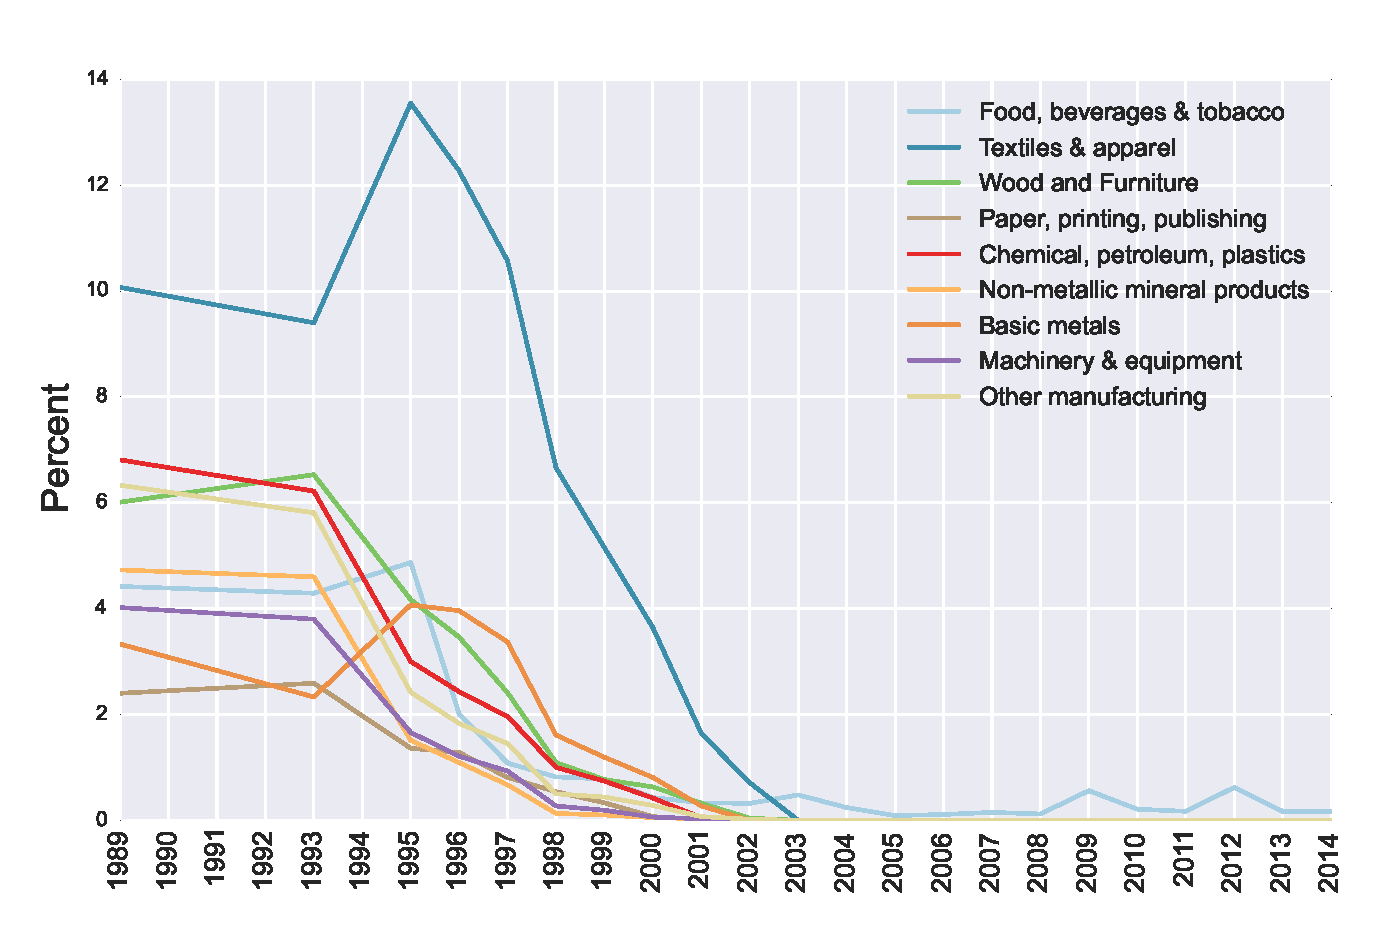
\includegraphics[scale=0.5]{tau_can_mex}
\label{fig:can_mex}
\end{figure} 

\begin{figure}[htpb]\centering
\caption{Canadian Tariff on U.S. Goods}\vspace{0.2cm}
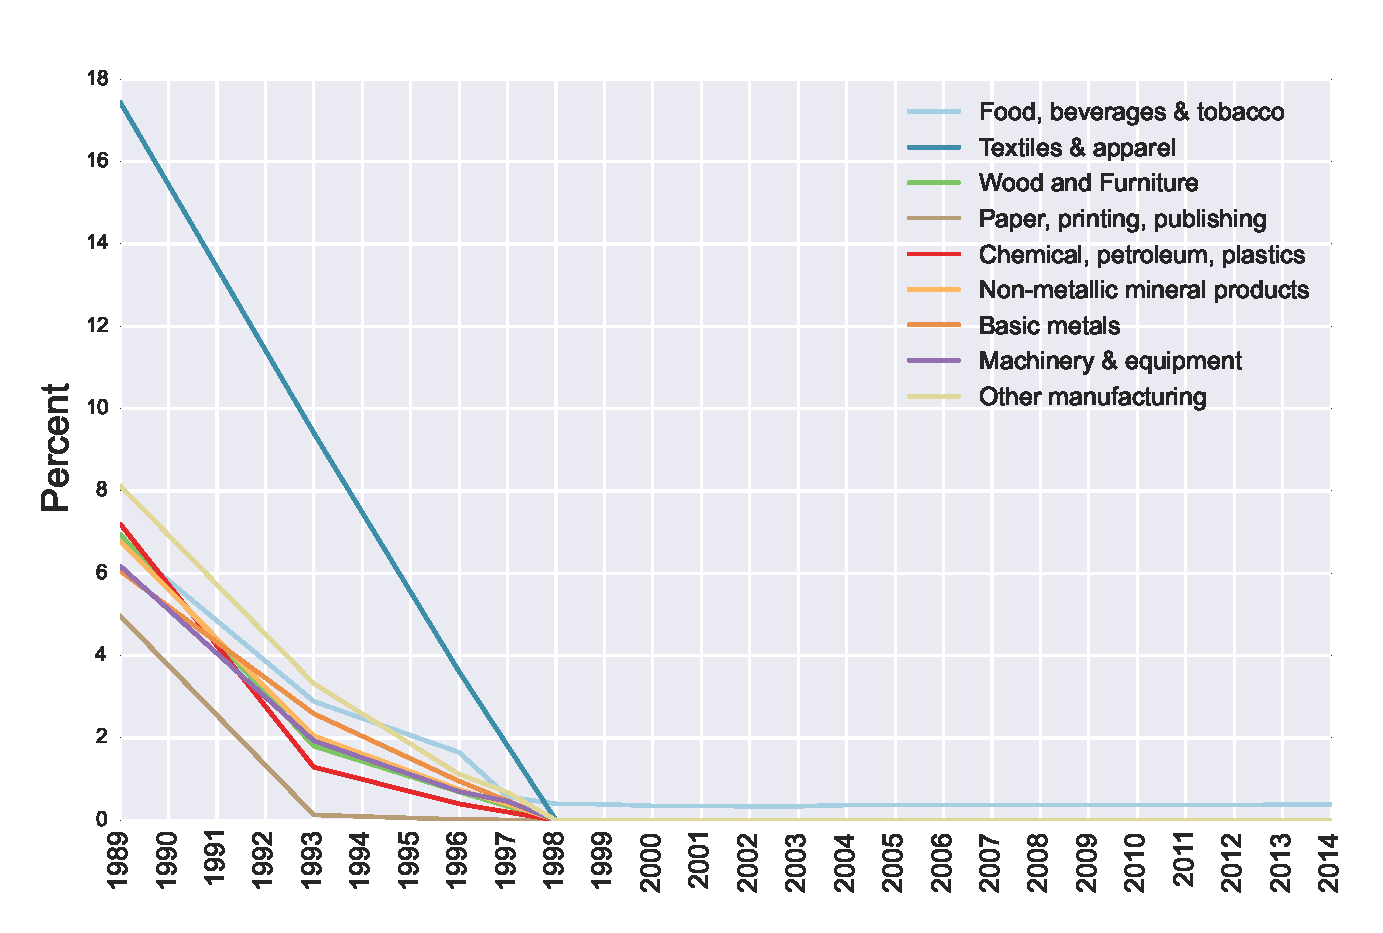
\includegraphics[scale=0.5]{tau_can_usa}
\label{fig:can_usa}
\end{figure}

\newpage

\begin{figure}[htpb]\centering
\caption{\small Mexican Tariff on Canadian Goods}\vspace{0.2cm}
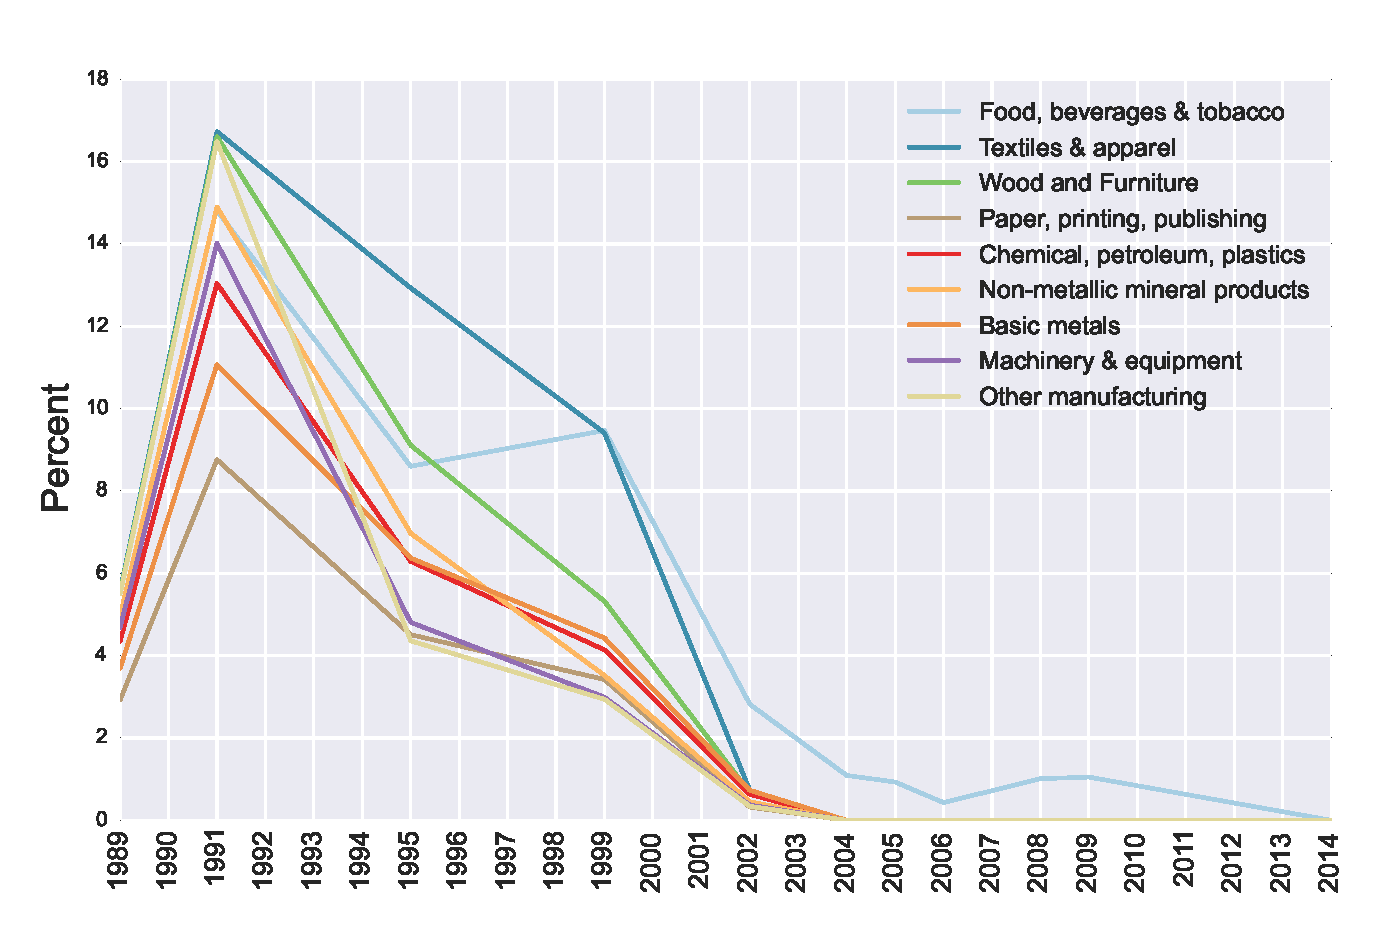
\includegraphics[scale=0.5]{tau_mex_can}
\label{fig:mex_can}
\end{figure}

\begin{figure}[htpb]\centering
\caption{\small Mexican Tariff on U.S. Goods}\vspace{0.2cm}
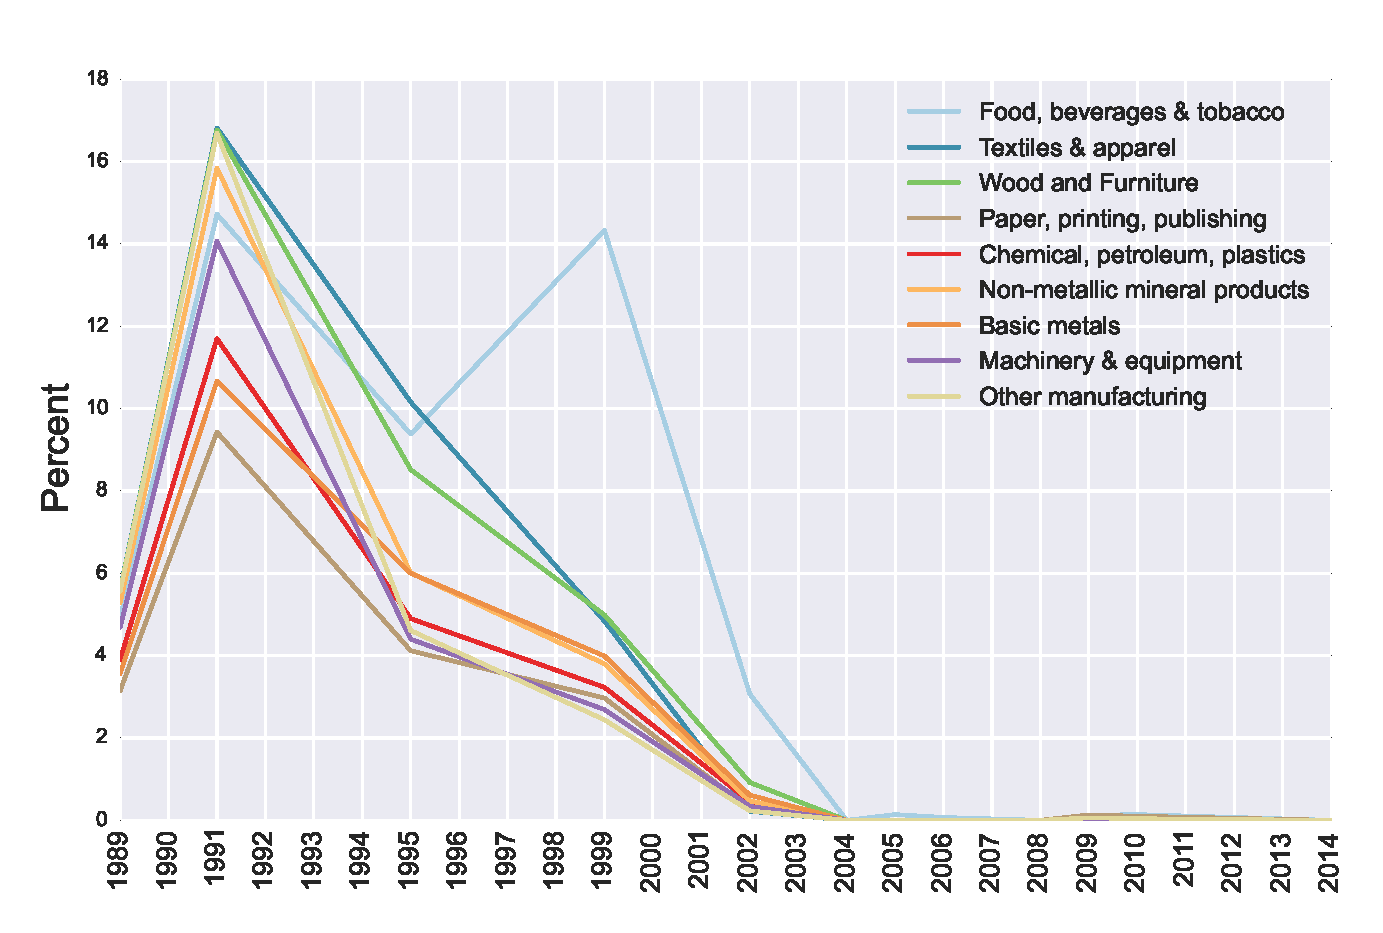
\includegraphics[scale=0.5]{tau_mex_usa}
\label{fig:mex_usa}
\end{figure}

\newpage

\begin{figure}[htpb]\centering
\caption{\small U.S. Tariff on Canadian Goods}\vspace{0.2cm}
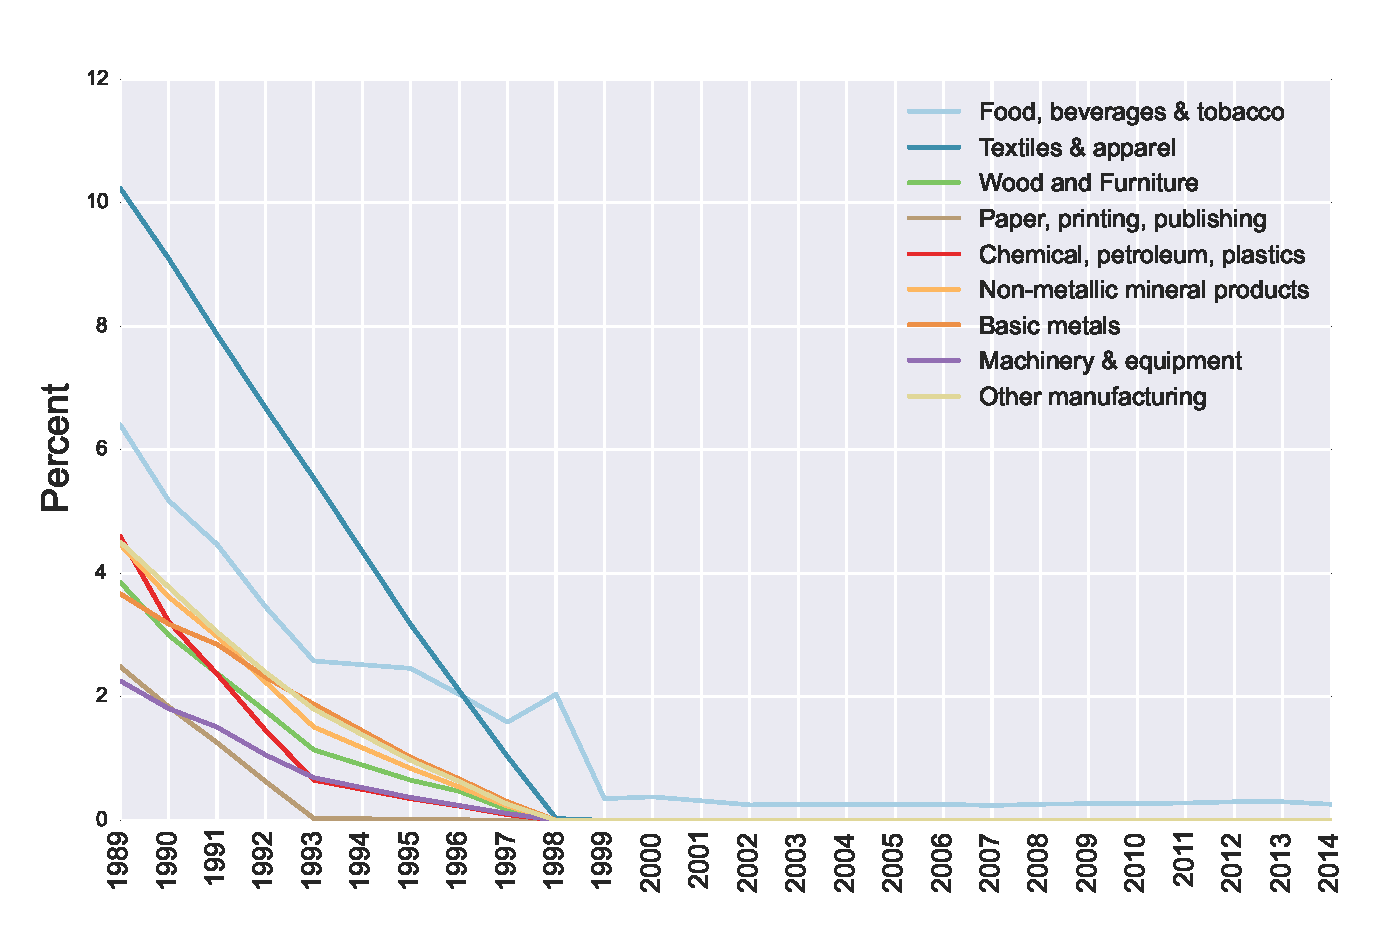
\includegraphics[scale=0.5]{tau_usa_can}
\label{fig:usa_can}
\end{figure}
 
\begin{figure}[htpb]\centering
\caption{\small U.S. Tariff on Mexican Goods}\vspace{0.2cm}
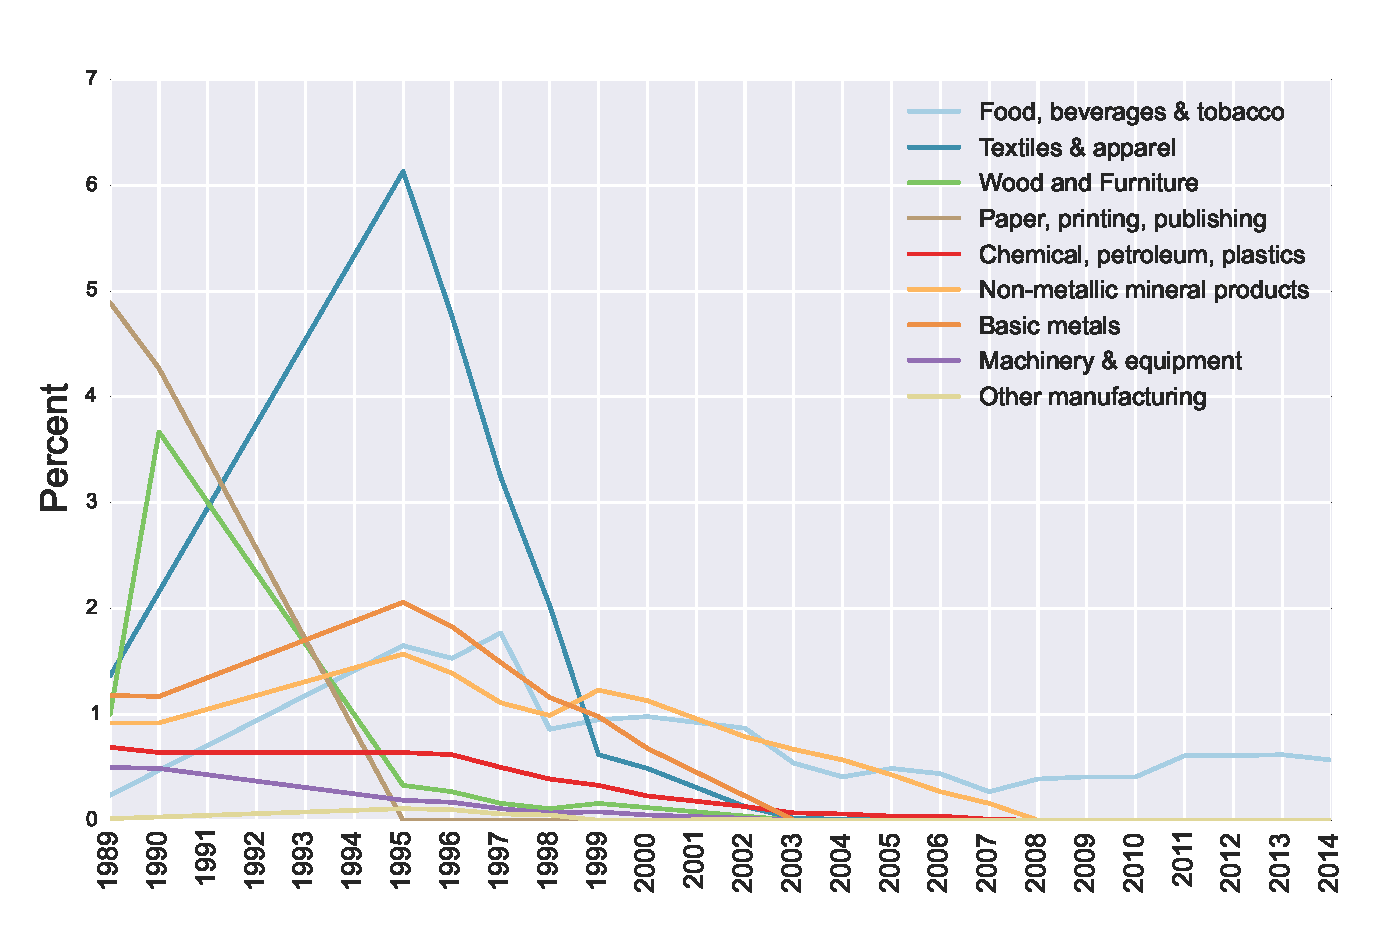
\includegraphics[scale=0.5]{tau_usa_mex}
\label{fig:usa_mex}
\end{figure}


\begin{center}
\begin{sidewaystable}

% Table created by stargazer v.5.0 by Marek Hlavac, Harvard University. E-mail: hlavac at fas.harvard.edu
% Date and time: Mon, Apr 28, 2014 - 18:37:50
% Requires LaTeX packages: rotating 
\begin{tabular}{@{\extracolsep{5pt}}lccccc} 
\\[-1.8ex]\hline 
\hline \\[-1.8ex] 
Statistic & \multicolumn{1}{c}{N} & \multicolumn{1}{c}{Mean} & \multicolumn{1}{c}{St. Dev.} & \multicolumn{1}{c}{Min} & \multicolumn{1}{c}{Max} \\ 
exp\_f & 702 & 76,233,571,691.000 & 198,643,966,085.000 & 399,038,863 & 1,890,000,000,000 \\ 
gdp\_can & 594 & 908.568 & 278.187 & 536.500 & 1,370.640 \\ 
gdp\_mex & 594 & 1,036.795 & 315.456 & 560.660 & 1,566.310 \\ 
gdp\_usa & 594 & 9,807.745 & 2,991.049 & 5,482.130 & 14,498.930 \\ 
cpi\_can & 675 & 79.697 & 12.487 & 56.340 & 100.000 \\ 
cpi\_mex & 675 & 48.219 & 32.559 & 1.560 & 100.000 \\ 
cpi\_usa & 675 & 75.546 & 14.894 & 50.300 & 100.000 \\ 
open\_ind\_can & 810 & 59.378 & 12.446 & 37.550 & 75.580 \\ 
open\_ind\_mex & 810 & 34.822 & 17.307 & 13.210 & 62.320 \\ 
open\_ind\_usa & 810 & 22.673 & 3.691 & 17.190 & 30.970 \\ 
ppi\_mex & 810 & 57.485 & 51.438 & 0.100 & 276.590 \\ 
tau\_s\_can\_mex & 540 & 1.829 & 3.193 & 0.000 & 17.780 \\ 
tau\_s\_can\_usa & 540 & 2.440 & 5.051 & 0.000 & 26.440 \\ 
tau\_s\_mex\_can & 405 & 8.654 & 8.751 & 0.000 & 30.530 \\ 
tau\_s\_mex\_usa & 405 & 7.611 & 8.552 & 0.000 & 28.800 \\ 
tau\_s\_usa\_can & 621 & 0.994 & 1.780 & 0.000 & 10.600 \\ 
tau\_s\_usa\_mex & 621 & 1.717 & 2.654 & 0.000 & 11.810 \\ 
\hline \\[-1.8ex] 
\end{tabular} 

\caption{Summary Statistics}
\label{tab:sumstats}
\end{sidewaystable}
\end{center}
\footnote{The majority of output tables in this paper has been produced using the stargazer package \citep{Hlavac2014}}

\newpage

\section{Appendix B: Industry list, NAICS classification}

\begin{longtable}{cl}
\caption{Industry List, NAICS 4-digit}\label{tab:naics4diglist}
NAICS 4-digit & Industry \\
3111 &	Animal Food Manufacturing \\
3112 &	Grain and Oilseed Milling \\
3113 &	Sugar and Confectionery Product Manufacturing \\
3114 &	Fruit and Vegetable Preserving and Specialty Food Manufacturing \\
3115 &	Dairy Product Manufacturing \\
3116 &	Animal Slaughtering and Processing \\
3118 &	Bakeries and Tortilla Manufacturing \\
3119 &	Other Food Manufacturing \\
3121 &	Beverage Manufacturing \\
3132 &	Fabric Mills \\
3133 &	Textile and Fabric Finishing and Fabric Coating Mills \\
3149 &	Other Textile Product Mills \\
3152 &	Cut and Sew Apparel Manufacturing \\
3159 &	Apparel Accessories and Other Apparel Manufacturing \\
3169 &	Other Leather and Allied Product Manufacturing \\
3211 &	Sawmills and Wood Preservation \\
3212 &	Veneer, Plywood, and Engineered Wood Product Manufacturing \\
3219 &	Other Wood Product Manufacturing \\
3221 &	Pulp, Paper, and Paperboard Mills \\
3222 &	Converted Paper Product Manufacturing \\
3231 &	Printing and Related Support Activities \\
3241 &	Petroleum and Coal Products Manufacturing \\
3251 &	Basic Chemical Manufacturing \\
3254 &	Pharmaceutical and Medicine Manufacturing \\
3255 &	Paint, Coating, and Adhesive Manufacturing \\
3256 &	Soap, Cleaning Compound, and Toilet Preparation Manufacturing \\
3259 &	Other Chemical Product and Preparation Manufacturing \\
3262 &	Rubber Product Manufacturing \\
3271 &	Clay Product and Refractory Manufacturing \\
3273 &	Cement and Concrete Product Manufacturing \\
3274 &	Lime and Gypsum Product Manufacturing \\
3279 &	Other Nonmetallic Mineral Product Manufacturing \\
3312 &	Steel Product Manufacturing from Purchased Steel \\
3313 &	Alumina and Aluminum Production and Processing \\
3314 &	Nonferrous Metal (except Aluminum) Production and Processing \\
3315 &	Foundries \\
3321 &	Forging and Stamping \\
3322 &	Cutlery and Handtool Manufacturing \\
3323 &	Architectural and Structural Metals Manufacturing \\
3324 &	Boiler, Tank, and Shipping Container Manufacturing \\
3325 &	Hardware Manufacturing \\
3326 &	Spring and Wire Product Manufacturing \\
3327 &	Machine Shops; Turned Product; and Screw, Nut, and Bolt Manufacturing \\
3329 &	Other Fabricated Metal Product Manufacturing \\
3331 &	Agriculture, Construction, and Mining Machinery Manufacturing \\
3332 &	Industrial Machinery Manufacturing \\
3333 &	Commercial and Service Industry Machinery Manufacturing \\
3334 &	Ventilation, Heating, Air-Conditioning, \& Commercial Refrig. Eq. Manuf. \\
3335 &	Metalworking Machinery Manufacturing \\
3336 &	Engine, Turbine, and Power Transmission Equipment Manufacturing \\
3339 &	Other General Purpose Machinery Manufacturing \\
3342 &	Communications Equipment Manufacturing \\
3344 &	Semiconductor and Other Electronic Component Manufacturing \\
3345 &	Navigational, Measuring, Electromedical, and Control Instrum. Manuf. \\
3351 &	Electric Lighting Equipment Manufacturing \\
3352 &	Household Appliance Manufacturing \\
3353 &	Electrical Equipment Manufacturing \\
3359 &	Other Electrical Equipment and Component Manufacturing \\
3362 &	Motor Vehicle Body and Trailer Manufacturing \\
3363 &	Motor Vehicle Parts Manufacturing \\
3371 &	Household and Institutional Furniture and Kitchen Cabinet Manufacturing \\
3372 &	Office Furniture (including Fixtures) Manufacturing \\
3379 &	Other Furniture Related Product Manufacturing \\
3399 &	Other Miscellaneous Manufacturing \\
\end{longtable}

%\begin{center}
%\begin{table*}[ht] \caption{Manufacturing Sectors: ISIC Rev. 3 to ISIC Rev. 2 Conversion}\label{tb:isic_class}
%{\small 
%\hfill{}
%\begin{tabular}{| p{8cm} | p{8cm} |} 
%\hline
%\textbf{ISIC Rev. 3}&\textbf{ISIC Rev. 2}\\
%\hline
%\hline
%D15: Foods, products, and beverages &  31: Food, beverages, and tobacco\\
%D16: Tobacco products & \\
%\hline
%D17: Textiles & \\
%D18: Wearing apparel, dressing and dyeing of fur & 32: Textile, wearing apparel, and leather industries\\
%D19: Tanning and dressing of leather, manufacture of luggage, handbags, saddlery, harness and footwear & \\
%\hline
%D20: Wood and of products of wood and cork, except furniture; manufacture of articles of straw and plaiting materials & 33:Wood and Wood Products, Including Furniture\\
%\hline
%D21: Paper and paper products & 34: Paper and paper products, printing and publishing\\ 
%D22: Publishing, printing, and reproduction of recorded media & \\
%\hline
%D23: Coke, refined petroleum products and nuclear fuel & \\
%D24: Chemicals and chemical products & 35: Chemical, petroleum, coal, rubber and plastic products\\
%D25: Rubber and plastics products & \\
%\hline
%D26: Other non-metallic mineral products & 36: Non-metallic mineral products, except products of petroleum and coal\\
%\hline
%D27: Basic metals & 37: Basic Metal Industries\\
%\hline
%D28: Fabricated metal products, except machinery and equipment & \\
%D29: Machinery and equipment n.e.c. & \\
%D30: Office, accounting and computing machinery & \\
%D31: Electrical machinery and apparatus n.e.c. & 38: Fabricated metal products, machinery and equipment\\
%D32: Radio, television and communication equipment and apparatus & \\
%D33: Medical, precision and optical instruments, watches and clocks & \\
%D34: Motor vehicles, trailers and semi-trailers & \\
%D35: Other transport equipment & \\
%\hline
%D36: Manufacture of furniture; manufacturing n.e.c. & 39: Other Manufacturing Industries\\
%D37: Recycling & \\
%\hline
%\end{tabular}}
%\end{table*}
%\end{center}

\section{Appendix C: Regression Results}

\begin{table}
\tiny
\begin{center}\caption{Prices (Short Run), all country pairs\label{tb:prices_sr}}

% Table created by stargazer v.5.0 by Marek Hlavac, Harvard University. E-mail: hlavac at fas.harvard.edu
% Date and time: Mon, Apr 28, 2014 - 18:47:21
\begin{tabular}{@{\extracolsep{5pt}}lcc} 
\\[-1.8ex]\hline 
\hline \\[-1.8ex] 
 & \multicolumn{2}{c}{\textit{Dependent variable:}} \\ 
\cline{2-3} 
\\[-1.8ex] & \multicolumn{2}{c}{$\Delta \log \left(\frac{p}{p^*} \right)$} \\ 
\\[-1.8ex] & (1) & (2)\\ 
\hline \\[-1.8ex] 
 $\Delta \log \tau_t$ & 0.002 & 0.002 \\ 
  & (0.002) & (0.002) \\ 
  & & \\ 
 $\Delta \log \tau_t^*$ & $-$0.003$^{*}$ & $-$0.003 \\ 
  & (0.002) & (0.002) \\ 
  & & \\ 
 $\Delta \log \theta_t$ & $-$0.106$^{***}$ & $-$0.104$^{***}$ \\ 
  & (0.014) & (0.015) \\ 
  & & \\ 
 $\Delta \log \theta_t^*$ & 0.247$^{***}$ & 0.248$^{***}$ \\ 
  & (0.023) & (0.024) \\ 
  & & \\ 
 $\Delta \log D_t$ & 0.015 & 0.016 \\ 
  & (0.025) & (0.025) \\ 
  & & \\ 
 $\Delta \log D_t^*$ & $-$0.034 & $-$0.084 \\ 
  & (0.134) & (0.153) \\ 
  & & \\ 
\hline \\[-1.8ex] 
Observations & 320 & 320 \\ 
R$^{2}$ & 0.371 & 0.379 \\ 
\hline 
\hline \\[-1.8ex] 
\textit{Note:}  & \multicolumn{2}{r}{$^{*}$p$<$0.1; $^{**}$p$<$0.05; $^{***}$p$<$0.01} \\ 
 & \multicolumn{2}{r}{Fixed effects for country pair} \\ 
\end{tabular} 

\end{center}
\end{table}

\begin{table}
\tiny
\begin{center}\caption{Prices (Short Run), all country pairs\label{tb:prices_sr}}

% Table created by stargazer v.5.1 by Marek Hlavac, Harvard University. E-mail: hlavac at fas.harvard.edu
% Date and time: Fri, Oct 02, 2015 - 00:31:10
\begin{tabular}{@{\extracolsep{5pt}}lcccccc} 
\\[-1.8ex]\hline 
\hline \\[-1.8ex] 
 & \multicolumn{6}{c}{\textit{Dependent variable:}} \\ 
\cline{2-7} 
\\[-1.8ex] & \multicolumn{6}{c}{$\Delta \log \left(\frac{p}{p^*} \right)$} \\ 
\\[-1.8ex] & (1) & (2) & (3) & (4) & (5) & (6)\\ 
\hline \\[-1.8ex] 
 $\Delta \log \tau^{hf}$ & $-$0.003 & 0.003 &  & $-$0.004 &  &  \\ 
  & (0.009) & (0.008) &  & (0.013) &  &  \\ 
  & & & & & & \\ 
 $\Delta \log \tau^{fh}$ & 0.003 & 0.003 & 0.161 & 0.004 & $-$0.061 & $-$0.061 \\ 
  & (0.004) & (0.005) & (0.182) & (0.007) & (0.084) & (0.084) \\ 
  & & & & & & \\ 
 $\Delta \log \tau^{ht}$ & 0.030 & 0.002 &  & 0.036 &  &  \\ 
  & (0.023) & (0.019) &  & (0.034) &  &  \\ 
  & & & & & & \\ 
 $\Delta \log \tau^{th}$ & 0.010$^{**}$ & 0.007 &  & 0.013$^{*}$ &  &  \\ 
  & (0.004) & (0.005) &  & (0.007) &  &  \\ 
  & & & & & & \\ 
 $\Delta \log \tau^{ft}$ & $-$0.002 & $-$0.001 & 0.055 & $-$0.002 & $-$0.045 & $-$0.045 \\ 
  & (0.004) & (0.005) & (0.182) & (0.007) & (0.084) & (0.084) \\ 
  & & & & & & \\ 
 $\Delta \log \tau^{tf}$ & 0.006 & 0.007 & $-$0.106 & 0.008 & 0.015 & 0.015 \\ 
  & (0.006) & (0.007) & (0.182) & (0.009) & (0.084) & (0.084) \\ 
  & & & & & & \\ 
 $\Delta \log D_t$ & 0.015 & 0.022 & 0.017 & $-$0.034 & 0.013 & 0.013 \\ 
  & (0.019) & (0.024) & (0.015) & (0.112) & (0.022) & (0.022) \\ 
  & & & & & & \\ 
 $\Delta \log D_t^*$ & $-$0.018 & $-$0.010 & $-$0.018 & 0.950 & $-$0.016 & $-$0.016 \\ 
  & (0.020) & (0.026) & (0.016) & (0.645) & (0.022) & (0.022) \\ 
  & & & & & & \\ 
\hline \\[-1.8ex] 
Observations & 364 & 364 & 134 & 118 & 134 & 134 \\ 
R$^{2}$ & 0.062 & 0.012 & 0.056 & 0.127 & 0.013 & 0.013 \\ 
\hline 
\hline \\[-1.8ex] 
\textit{Note:}  & \multicolumn{6}{r}{$^{*}$p$<$0.1; $^{**}$p$<$0.05; $^{***}$p$<$0.01} \\ 
 & \multicolumn{6}{r}{(1),(3): Fixed effects country-industry: (2),(4): Fixed effects country pair} \\ 
\end{tabular} 

\end{center}
\end{table}

\begin{table}
\tiny
\begin{center}\caption{Prices (Short Run), all country pairs\label{tb:prices_sr}}

% Table created by stargazer v.5.1 by Marek Hlavac, Harvard University. E-mail: hlavac at fas.harvard.edu
% Date and time: Fri, Oct 02, 2015 - 00:22:45
\begin{tabular}{@{\extracolsep{5pt}}lcccccc} 
\\[-1.8ex]\hline 
\hline \\[-1.8ex] 
 & \multicolumn{6}{c}{\textit{Dependent variable:}} \\ 
\cline{2-7} 
\\[-1.8ex] & \multicolumn{6}{c}{$\Delta \log \left(\frac{p}{p^*} \right)$} \\ 
\\[-1.8ex] & (1) & (2) & (3) & (4) & (5) & (6)\\ 
\hline \\[-1.8ex] 
 $\Delta \log \tau_t$ & 0.0002 & 0.0003 & $-$0.003 & 0.002 & $-$0.003 & 0.002 \\ 
  & (0.001) & (0.002) & (0.003) & (0.003) & (0.003) & (0.003) \\ 
  & & & & & & \\ 
 $\Delta \log \tau_t^*$ & $-$0.003$^{**}$ & $-$0.004$^{**}$ & $-$0.002 & $-$0.004 & $-$0.002 & $-$0.004 \\ 
  & (0.002) & (0.002) & (0.003) & (0.003) & (0.003) & (0.003) \\ 
  & & & & & & \\ 
 $\Delta \log D_t$ & 0.012 & 0.013$^{*}$ & 0.010 & 0.018 & 0.010 & 0.018 \\ 
  & (0.007) & (0.008) & (0.009) & (0.020) & (0.009) & (0.020) \\ 
  & & & & & & \\ 
 $\Delta \log D_t^*$ & $-$0.019 & $-$0.013 & $-$0.017 & $-$0.186 & $-$0.017 & $-$0.186 \\ 
  & (0.023) & (0.023) & (0.019) & (0.266) & (0.019) & (0.266) \\ 
  & & & & & & \\ 
\hline \\[-1.8ex] 
Observations & 984 & 984 & 354 & 318 & 354 & 318 \\ 
R$^{2}$ & 0.012 & 0.009 & 0.033 & 0.010 & 0.033 & 0.010 \\ 
\hline 
\hline \\[-1.8ex] 
\textit{Note:}  & \multicolumn{6}{r}{$^{*}$p$<$0.1; $^{**}$p$<$0.05; $^{***}$p$<$0.01} \\ 
 & \multicolumn{6}{r}{(1),(3): Fixed effects country-industry (2),(4): Fixed effects country pair} \\ 
\end{tabular} 

\end{center}
\end{table}

\begin{table}
\tiny
\begin{center}\caption{Markups (Short Run), all country pairs\label{tb:markup_sr}}

% Table created by stargazer v.5.0 by Marek Hlavac, Harvard University. E-mail: hlavac at fas.harvard.edu
% Date and time: Thu, Apr 24, 2014 - 19:57:37
\begin{tabular}{@{\extracolsep{5pt}}lcccc} 
\\[-1.8ex]\hline 
\hline \\[-1.8ex] 
 & \multicolumn{4}{c}{\textit{Dependent variable:}} \\ 
\cline{2-5} 
\\[-1.8ex] & \multicolumn{4}{c}{$\Delta \log \left(\frac{\mu}{\mu^*} \right)$} \\ 
\\[-1.8ex] & (1) & (2) & (3) & (4)\\ 
\hline \\[-1.8ex] 
 $\Delta \log \tau_t$ & 0.001 & 0.001 & 0.001 & 0.001 \\ 
  & (0.001) & (0.001) & (0.001) & (0.001) \\ 
  & & & & \\ 
 $\Delta \log \tau_t^*$ & 0.00003 & 0.00003 & 0.0002 & 0.0002 \\ 
  & (0.001) & (0.001) & (0.001) & (0.001) \\ 
  & & & & \\ 
 $\Delta \log \theta$ &  &  & $-$0.024$^{***}$ & $-$0.024$^{***}$ \\ 
  &  &  & (0.005) & (0.006) \\ 
  & & & & \\ 
 $\Delta \log \theta^*$ &  &  & 0.028$^{***}$ & 0.028$^{***}$ \\ 
  &  &  & (0.009) & (0.009) \\ 
  & & & & \\ 
 $\Delta \log D_{t}$ & $-$0.003 & $-$0.002 & $-$0.005 & $-$0.003 \\ 
  & (0.009) & (0.009) & (0.009) & (0.009) \\ 
  & & & & \\ 
 $\Delta \log D_{t-1}$ & 0.049 & 0.006 & 0.037 & $-$0.008 \\ 
  & (0.050) & (0.056) & (0.049) & (0.055) \\ 
  & & & & \\ 
\hline \\[-1.8ex] 
Observations & 306 & 306 & 302 & 302 \\ 
R$^{2}$ & 0.009 & 0.006 & 0.109 & 0.107 \\ 
\hline 
\hline \\[-1.8ex] 
\textit{Note:}  & \multicolumn{4}{r}{$^{*}$p$<$0.1; $^{**}$p$<$0.05; $^{***}$p$<$0.01} \\ 
 & \multicolumn{4}{r}{Fixed effects for country pair} \\ 
\end{tabular} 

\end{center}
\end{table}

\begin{table}
\tiny
\begin{center} \caption{Productivity (Short Run), all country pairs\label{tb:productivity_sr}}

% Table created by stargazer v.5.1 by Marek Hlavac, Harvard University. E-mail: hlavac at fas.harvard.edu
% Date and time: Fri, Oct 02, 2015 - 13:51:58
\begin{tabular}{@{\extracolsep{5pt}}lcccccc} 
\\[-1.8ex]\hline 
\hline \\[-1.8ex] 
 & \multicolumn{6}{c}{\textit{Dependent variable:}} \\ 
\cline{2-7} 
\\[-1.8ex] & \multicolumn{6}{c}{$\Delta \log \left(\frac{z}{z^*} \right)$} \\ 
\\[-1.8ex] & (1) & (2) & (3) & (4) & (5) & (6)\\ 
\hline \\[-1.8ex] 
 $\Delta \log \tau_t$ & $-$0.009$^{***}$ & $-$0.009$^{***}$ & $-$0.018$^{***}$ & $-$0.002 & $-$0.018$^{***}$ & $-$0.002 \\ 
  & (0.003) & (0.003) & (0.005) & (0.006) & (0.005) & (0.006) \\ 
  & & & & & & \\ 
 $\Delta \log \tau_t^*$ & 0.006$^{*}$ & 0.006$^{*}$ & 0.010$^{**}$ & 0.011$^{*}$ & 0.010$^{**}$ & 0.011$^{*}$ \\ 
  & (0.003) & (0.003) & (0.004) & (0.006) & (0.004) & (0.006) \\ 
  & & & & & & \\ 
 $\Delta \log D_t$ & 0.146$^{***}$ & 0.145$^{***}$ & 0.200$^{***}$ & 0.056 & 0.201$^{***}$ & 0.051 \\ 
  & (0.056) & (0.054) & (0.072) & (0.118) & (0.070) & (0.114) \\ 
  & & & & & & \\ 
 $\Delta \log D_t^*$ & 0.015 & 0.035 & $-$0.097 & 0.541 & $-$0.095 & 0.716$^{*}$ \\ 
  & (0.089) & (0.083) & (0.091) & (0.484) & (0.088) & (0.399) \\ 
  & & & & & & \\ 
\hline \\[-1.8ex] 
Observations & 2,695 & 2,695 & 990 & 860 & 990 & 860 \\ 
R$^{2}$ & 0.007 & 0.006 & 0.022 & 0.006 & 0.021 & 0.008 \\ 
\hline 
\hline \\[-1.8ex] 
\textit{Note:}  & \multicolumn{6}{r}{$^{*}$p$<$0.1; $^{**}$p$<$0.05; $^{***}$p$<$0.01} \\ 
 & \multicolumn{6}{r}{(1),(3),(4): Fixed effects country-industry; (2),(5),(6): Fixed effect country pair} \\ 
\end{tabular} 

\end{center}
\end{table}

\begin{table}
\tiny
\begin{center}\caption{Prices (Long Run), all country pairs\label{tb:prices_lr}}

% Table created by stargazer v.5.1 by Marek Hlavac, Harvard University. E-mail: hlavac at fas.harvard.edu
% Date and time: Fri, Oct 02, 2015 - 13:14:33
\begin{tabular}{@{\extracolsep{5pt}}lcccccc} 
\\[-1.8ex]\hline 
\hline \\[-1.8ex] 
 & \multicolumn{6}{c}{\textit{Dependent variable:}} \\ 
\cline{2-7} 
\\[-1.8ex] & \multicolumn{6}{c}{$\Delta \log \left(\frac{p_t}{p_t^*} \right)$} \\ 
\\[-1.8ex] & (1) & (2) & (3) & (4) & (5) & (6)\\ 
\hline \\[-1.8ex] 
 $\Delta \log \tau_t$ & 0.001 & 0.001 & $-$0.001 & 0.005$^{**}$ & $-$0.001 & 0.004$^{**}$ \\ 
  & (0.001) & (0.001) & (0.002) & (0.002) & (0.002) & (0.002) \\ 
  & & & & & & \\ 
 $\Delta \log \tau_t^*$ & $-$0.001 & 0.00004 & $-$0.00004 & $-$0.002 & 0.0002 & 0.0004 \\ 
  & (0.001) & (0.001) & (0.002) & (0.002) & (0.002) & (0.002) \\ 
  & & & & & & \\ 
 $\Delta \log D_t$ & $-$0.031 & $-$0.025 & $-$0.063$^{**}$ & 0.008 & $-$0.061$^{**}$ & 0.023 \\ 
  & (0.023) & (0.021) & (0.031) & (0.041) & (0.030) & (0.040) \\ 
  & & & & & & \\ 
 $\Delta \log D_t^*$ & 0.038 & 0.028 & 0.038 & 0.366$^{**}$ & 0.036 & 0.132 \\ 
  & (0.036) & (0.033) & (0.039) & (0.174) & (0.037) & (0.141) \\ 
  & & & & & & \\ 
 $\log \left(\frac{p_{t-1}}{p_{t-1}^*} \right)$ & $-$0.123$^{***}$ & $-$0.118$^{***}$ & $-$0.121$^{***}$ & $-$0.149$^{***}$ & $-$0.118$^{***}$ & $-$0.137$^{***}$ \\ 
  & (0.006) & (0.005) & (0.010) & (0.010) & (0.009) & (0.009) \\ 
  & & & & & & \\ 
 $\log \tau_{t-1}$ & $-$0.001 & $-$0.001 & $-$0.001 & $-$0.0003 & $-$0.001 & $-$0.001 \\ 
  & (0.001) & (0.001) & (0.002) & (0.002) & (0.002) & (0.002) \\ 
  & & & & & & \\ 
 $\log \tau_{t-1}^*$ & $-$0.002 & $-$0.00002 & $-$0.0003 & $-$0.006$^{***}$ & 0.0004 & $-$0.002 \\ 
  & (0.001) & (0.001) & (0.002) & (0.002) & (0.002) & (0.001) \\ 
  & & & & & & \\ 
 $\log L_{t-1}$ & $-$0.570$^{***}$ & $-$0.541$^{***}$ & $-$0.497$^{***}$ & $-$0.775$^{***}$ & $-$0.480$^{***}$ & $-$0.734$^{***}$ \\ 
  & (0.082) & (0.077) & (0.136) & (0.139) & (0.131) & (0.135) \\ 
  & & & & & & \\ 
 $\log L_{t-1}^*$ & 0.466$^{***}$ & 0.458$^{***}$ & 0.400$^{***}$ & 0.611$^{***}$ & 0.396$^{***}$ & 0.616$^{***}$ \\ 
  & (0.080) & (0.076) & (0.132) & (0.138) & (0.126) & (0.133) \\ 
  & & & & & & \\ 
\hline \\[-1.8ex] 
Observations & 2,769 & 2,769 & 1,021 & 881 & 1,021 & 881 \\ 
R$^{2}$ & 0.184 & 0.181 & 0.192 & 0.246 & 0.187 & 0.224 \\ 
\hline 
\hline \\[-1.8ex] 
\textit{Note:}  & \multicolumn{6}{r}{$^{*}$p$<$0.1; $^{**}$p$<$0.05; $^{***}$p$<$0.01} \\ 
 & \multicolumn{6}{r}{Fixed effects for country pair} \\ 
\end{tabular} 

\end{center}
\end{table}


\begin{table}
\tiny
\begin{center}\caption{Markups (Long Run), all country pairs\label{tb:markup_lr}}

% Table created by stargazer v.5.0 by Marek Hlavac, Harvard University. E-mail: hlavac at fas.harvard.edu
% Date and time: Thu, Apr 24, 2014 - 19:57:52
\begin{tabular}{@{\extracolsep{5pt}}lcccc} 
\\[-1.8ex]\hline 
\hline \\[-1.8ex] 
 & \multicolumn{4}{c}{\textit{Dependent variable:}} \\ 
\cline{2-5} 
\\[-1.8ex] & \multicolumn{4}{c}{$\Delta \log \left(\frac{\mu}{\mu^*} \right)$} \\ 
\\[-1.8ex] & (1) & (2) & (3) & (4)\\ 
\hline \\[-1.8ex] 
 $\Delta \log \tau$ & 0.001 & 0.0004 & 0.001 & 0.0005 \\ 
  & (0.001) & (0.001) & (0.001) & (0.001) \\ 
  & & & & \\ 
 $\Delta \log \tau^*$ & 0.001 & 0.001 & 0.00002 & 0.0003 \\ 
  & (0.001) & (0.001) & (0.001) & (0.001) \\ 
  & & & & \\ 
 $\Delta \log \theta$ &  &  & $-$0.032$^{***}$ & $-$0.027$^{***}$ \\ 
  &  &  & (0.006) & (0.006) \\ 
  & & & & \\ 
 $\Delta \log \theta^*$ &  &  & 0.048$^{***}$ & 0.095$^{***}$ \\ 
  &  &  & (0.010) & (0.016) \\ 
  & & & & \\ 
 $\Delta \log D_t$ & $-$0.0004 & 0.012 & $-$0.004 & 0.006 \\ 
  & (0.009) & (0.008) & (0.009) & (0.007) \\ 
  & & & & \\ 
 $\Delta \log D_t^*$ & 0.027 & $-$0.055 & 0.034 & $-$0.063 \\ 
  & (0.053) & (0.050) & (0.051) & (0.047) \\ 
  & & & & \\ 
 $\log \left(\frac{\mu_{t-1}}{\mu_{t-1}^*} \right)$ & 0.010 & $-$0.460$^{***}$ & 0.003 & $-$0.454$^{***}$ \\ 
  & (0.007) & (0.042) & (0.007) & (0.039) \\ 
  & & & & \\ 
 $\tau_{t-1}$ & $-$0.001 & $-$0.002$^{**}$ & $-$0.001 & $-$0.002$^{**}$ \\ 
  & (0.001) & (0.001) & (0.001) & (0.001) \\ 
  & & & & \\ 
 $\tau_{t-1}^*$ & 0.001 & 0.001$^{*}$ & $-$0.0001 & 0.001 \\ 
  & (0.001) & (0.001) & (0.001) & (0.001) \\ 
  & & & & \\ 
 $\log \theta_{t-1}$ &  &  & $-$0.010$^{***}$ & $-$0.010$^{*}$ \\ 
  &  &  & (0.003) & (0.005) \\ 
  & & & & \\ 
 $\log \theta_{t-1}^*$ &  &  & 0.008$^{**}$ & 0.037$^{***}$ \\ 
  &  &  & (0.003) & (0.010) \\ 
  & & & & \\ 
 $L_{t-1}$ & $-$0.156$^{*}$ & $-$0.128$^{*}$ & $-$0.255$^{***}$ & $-$0.185$^{***}$ \\ 
  & (0.080) & (0.068) & (0.080) & (0.066) \\ 
  & & & & \\ 
 $L_{t-1}^*$ & 0.139$^{*}$ & 0.104 & 0.230$^{***}$ & 0.138$^{**}$ \\ 
  & (0.081) & (0.068) & (0.081) & (0.068) \\ 
  & & & & \\ 
\hline \\[-1.8ex] 
Observations & 306 & 306 & 302 & 302 \\ 
R$^{2}$ & 0.040 & 0.332 & 0.183 & 0.491 \\ 
\hline 
\hline \\[-1.8ex] 
\textit{Note:}  & \multicolumn{4}{r}{$^{*}$p$<$0.1; $^{**}$p$<$0.05; $^{***}$p$<$0.01} \\ 
 & \multicolumn{4}{r}{Fixed effects for country pair} \\ 
\end{tabular} 

\end{center}
\end{table}

\begin{table}
\tiny
\begin{center}\caption{Productivity (Long Run), all country pairs\label{tb:productivity_lr}}

% Table created by stargazer v.5.0 by Marek Hlavac, Harvard University. E-mail: hlavac at fas.harvard.edu
% Date and time: Thu, Apr 24, 2014 - 19:57:58
\begin{tabular}{@{\extracolsep{5pt}}lcccc} 
\\[-1.8ex]\hline 
\hline \\[-1.8ex] 
 & \multicolumn{4}{c}{\textit{Dependent variable:}} \\ 
\cline{2-5} 
\\[-1.8ex] & \multicolumn{4}{c}{$\Delta \log \left(\frac{z}{z^*} \right)$} \\ 
\\[-1.8ex] & (1) & (2) & (3) & (4)\\ 
\hline \\[-1.8ex] 
 $\Delta \log \tau_t$ & 0.0002 & $-$0.001 & 0.004 & 0.003 \\ 
  & (0.005) & (0.004) & (0.004) & (0.004) \\ 
  & & & & \\ 
 $\Delta \log \tau_t^*$ & 0.001 & 0.004 & $-$0.001 & 0.002 \\ 
  & (0.005) & (0.005) & (0.005) & (0.005) \\ 
  & & & & \\ 
 $\Delta \log \theta$ &  &  & $-$0.245$^{***}$ & $-$0.214$^{***}$ \\ 
  &  &  & (0.040) & (0.042) \\ 
  & & & & \\ 
 $\Delta \log \theta^*$ &  &  & 0.574$^{***}$ & 0.451$^{***}$ \\ 
  &  &  & (0.070) & (0.131) \\ 
  & & & & \\ 
 $\Delta \log D_t$ & $-$0.428$^{*}$ & 0.409$^{*}$ & $-$0.179 & 0.262 \\ 
  & (0.246) & (0.221) & (0.210) & (0.208) \\ 
  & & & & \\ 
 $\Delta \log D_t^*$ & 0.336 & $-$0.427 & 0.167 & $-$0.175 \\ 
  & (0.393) & (0.358) & (0.345) & (0.353) \\ 
  & & & & \\ 
 $\log \left(\frac{z_{t-1}}{z_{t-1}^*} \right)$ & $-$0.145$^{***}$ & $-$0.348$^{***}$ & $-$0.089$^{***}$ & $-$0.308$^{***}$ \\ 
  & (0.016) & (0.022) & (0.015) & (0.033) \\ 
  & & & & \\ 
 $\log \tau_{t-1}$ & $-$0.008 & $-$0.009$^{*}$ & $-$0.007 & $-$0.006 \\ 
  & (0.006) & (0.005) & (0.005) & (0.005) \\ 
  & & & & \\ 
 $\log \tau_{t-1}^*$ & 0.006 & 0.013$^{**}$ & 0.0004 & 0.006 \\ 
  & (0.005) & (0.005) & (0.005) & (0.005) \\ 
  & & & & \\ 
 $\log \theta_{t-1}$ &  &  & $-$0.012 & $-$0.092$^{**}$ \\ 
  &  &  & (0.021) & (0.043) \\ 
  & & & & \\ 
 $\log \theta_{t-1}^*$ &  &  & $-$0.010 & 0.119 \\ 
  &  &  & (0.021) & (0.078) \\ 
  & & & & \\ 
 $\log L_{t-1}$ & 0.569 & $-$1.531$^{***}$ & $-$0.523 & $-$1.625$^{***}$ \\ 
  & (0.623) & (0.559) & (0.539) & (0.538) \\ 
  & & & & \\ 
 $\log L_{t-1}^*$ & $-$0.777 & 1.740$^{***}$ & 0.198 & 1.416$^{***}$ \\ 
  & (0.636) & (0.568) & (0.547) & (0.543) \\ 
  & & & & \\ 
 $\log w_{t-1}$ & 0.160$^{**}$ & 0.181$^{**}$ & 0.068 & 0.216$^{**}$ \\ 
  & (0.063) & (0.090) & (0.058) & (0.100) \\ 
  & & & & \\ 
 $\log w_{t-1}^*$ & $-$0.230$^{***}$ & $-$0.584$^{***}$ & $-$0.063 & $-$0.129 \\ 
  & (0.069) & (0.117) & (0.062) & (0.142) \\ 
  & & & & \\ 
\hline \\[-1.8ex] 
Observations & 324 & 324 & 320 & 320 \\ 
R$^{2}$ & 0.290 & 0.543 & 0.510 & 0.613 \\ 
\hline 
\hline \\[-1.8ex] 
\textit{Note:}  & \multicolumn{4}{r}{$^{*}$p$<$0.1; $^{**}$p$<$0.05; $^{***}$p$<$0.01} \\ 
 & \multicolumn{4}{r}{Fixed effects for country pair or industry/country pair} \\ 
\end{tabular} 

\end{center}
\end{table}

\section{Appendix D: Data Appendix}
\begin{spacing}{1}

\noindent \textbf{Tariffs ($\tau$)}
	\begin{itemize}
	
	\item \emph{Definition}: All tariff data is downloaded from the \href{http://wits.worldbank.org/Default.aspx}{World Integrated Trade Solution (WITS)}, an online software package published by the World Bank in collaboration with UNCTAD, the WTO, International Trade Center, and the UN Statistical Division. WITS publishes annual trade and tariff data from two different sources: the World Bank IDB database and the UNCTAD TRAINS database. Unfortunately, neither database provides a complete time series for each country that is devoid of erratic (and unexplained) jumps in the data. Thus, we created a data set that uses mostly TRAINS preferential tariff (PRF) data, but supplements it with observations from TRAINS or WTO IDB applied tariffs (AHS) where appropriate (this choice will only make a difference where there is no trade observed between countries and hence no applied rate, but a preferential rate still exists). All tariff data is reported according to ISIC Rev. 3.1 and converted to NAICS. This leads to the following rules for construction for each country:
		\begin{itemize}
		\item \underline{Canada}: TRAINS PRF from 1989 to 1995, WTO AHS from 1996 to 2014.

		\item \underline{Mexico}: TRAINS AHS from 1989 to 1994, TRAINS PRF from 1995 to 2009.

		\item \underline{USA}: TRAINS PRF from 1980 to 1996; WTO AHS for 1997 to 2014.
		\end{itemize}
	\end{itemize}


\noindent \textbf{Prices ($p$)}
	\begin{itemize}
	
	\item \emph{Definition}: The Producer Price Index (PPI) measures the average change over time in selling prices received by domestic producers of goods and services. This measure contrasts with the Consumer Price Index (CPI) which measures the price change from the perspective of the consumer. 
	
	\item \underline{USA}: Producer price index (PPI) reported by commodity and converted to the North American Industry Classification System (NAICS) using the Bureau of Labor Statistics' (BLS) concordance table (1988-2014, 2003=100). All industries with more than one PPI reported (due to multiple commodities matching the industry) are averaged. Source: \href{http://www.bls.gov/ppi/#data}{Bureau of Labor Statistics}. %Accessed: 17 September 2015.
		
	\item \underline{Canada}: Industrial product price indexes, by North American Industry Classification System (NAICS), annual (index, 2003=100), Table 329-0077, 1993-2014. Industry price indexes, by industry and industry group (reported according to SIC and converted to NAICS), annual (index, 1992=100), Table 329-0001, 1988-1992. Source: \href{http://www5.statcan.gc.ca/cansim/a47}{Statistics Canada}. %Accessed: 31 August 2015.

	\item \underline{Mexico}: Industrial producer price indices, total production by economic activity (ISIC Rev. 2), monthly (index, December 2003=100), 1988-2012. Monthly data are averaged to generate an annual price index, and ISIC Rev. 2 is converted to NAICS. Source: \href{http://www.inegi.org.mx/est/contenidos/proyectos/inp/INPP_CAB2003.aspx}{Instituto Nacional de Estadistica y Geografia}. %Accessed: 31 August 2015.
	
	\end{itemize}


%\noindent \textbf{Markups ($\mu$)}
%	\begin{itemize}
	
%	\item \emph{Definition}: We compute average markups as the ratio of sectoral turnover relative to total variable costs, which are computed as the sum of intermediate inputs and labor costs as reported by the OECD Structural Business Statistics (SDBS) database for all businesses (SSIS). Due to the unavailability of data on sectoral turnover, we use sectoral production as a proxy. While turnover may be slightly higher than production in a given year if all of the produced goods are sold along with any stored goods from previous years, according to the OECD these measures will converge in the long term. Fixed costs are excluded from the calculation, as they will cause a negative bias between markups and openness.
	
%	\item \textbf{Production}: Available for Canada (1990-2008), Mexico (1994-2007), and the {\color{red}U.S. (1997-2008) -- not available via NBER data; Ryan will check the 1992 Economic Census when received from library --} in current national currency (millions) from the \href{http://stats.oecd.org/index.aspx?queryid=224}{OECD SDBS database}. From the OECD SDBS database: ``The value of production corresponds to the sum of the value of all finished products (including intermediary products sold in the same condition as received), of the net change of the value of work in progress and stocks of goods to be shipped in the same condition as received, of the variation of stocks of finished products and of those in progress, of the value of goods or services rendered to others, of the value of goods shipped in the same condition as received less the amount paid for these goods and of the value of fixed assets produced by the unit for its own use.''
	
%	\item \textbf{Gross Operating Surplus}: Available for Canada (1990-2008); {\color{red}no data for Mexico or the US}. From the OECD SDBS database: ``Gross operating surplus is the surplus generated by operating activities after deducting labour costs (compensation of employees), and, depending on the valuation used for value added, taxes minus subsidies on production from value added. It reflects the balance available to the unit which allows it to recompense the providers of own funds and debt, to pay taxes and eventually to finance all or a part of its investment, and so measures the surplus or deficit accruing from production before taking account of any interest, rent or similar charges payable on financial or tangible non-produced assets borrowed or rented by the unit, or any interest, rent or similar receipts receivable on financial or tangible non-produced assets owned by the unit.''
	
%	\item \textbf{Wages and Salaries (employees)}: Available for Canada (1990-2008, ISIC Rev. 3.1) in current national currency (millions) from the \href{http://stats.oecd.org/index.aspx?queryid=224}{OECD SDBS database}; available for the U.S. (1988-2010, annually in nominal USD) from  the \href{http://www.nber.org/nberces/}{NBER-CES Manufacturing Industry Database} (Becker, Gray, and Marvakov, 2013).	 {\color{red}Mexico (1994-2003, missing 2001-2002)}, and {\color{red}the U.S. (1997-2008)} 
	
%	\end{itemize}

\noindent \textbf{Productivity ($z$)}
	\begin{itemize}
	
	\item \emph{Definition}: calculated as the ratio between real value-added and total employment, by manufacturing sector.
	
	\item \textbf{Value Added}:  Available for Canada (1990-2008, annually, millions of current CAD) from  the \href{http://stats.oecd.org/index.aspx?queryid=224}{OECD SDBS database}, Mexico (1988-2007, annually, millions of current MXN) from the Annual Industrial Survey (\emph{Encuesta Industrial Anual}), which is published annually by   the \href{http://buscador.inegi.org.mx/search?q=encuesta+industrial+anual&client=ProductosR&proxystylesheet=ProductosR&num=10&getfields=*&sort=meta:edicion:D:E:::D&entsp=a__inegi_politica_p72&lr=lang_es\%7Clang_en&oe=UTF-8&ie=UTF-8&ip=10.210.100.253&entqr=3&filter=0&site=ProductosBuscador&tlen=260&ulang=en&start=0}{\emph{Instituto Nacional de Estadistica y Geografia}}, and the U.S. (1988-2010, annually, millions of current USD) from  the \href{http://www.nber.org/nberces/}{NBER-CES Manufacturing Industry Database} (Becker, Gray, and Marvakov, 2013). All value added data is converted into constant 2003 USD.		
	
	\item \textbf{Employment}: Available for Canada (1990-2008, annually, ISIC Rev. 3) from the \href{http://stats.oecd.org/index.aspx?queryid=224}{OECD SDBS database},  Mexico (1988-1990, 1993, annual average, CMAP; 1994-1998, 2000-2007, annual average, ISIC Rev. 3.1) from the Annual Industrial Survey (\emph{Encuesta Industrial Anual}), which is published annually by   the \href{http://buscador.inegi.org.mx/search?q=encuesta+industrial+anual&client=ProductosR&proxystylesheet=ProductosR&num=10&getfields=*&sort=meta:edicion:D:E:::D&entsp=a__inegi_politica_p72&lr=lang_es\%7Clang_en&oe=UTF-8&ie=UTF-8&ip=10.210.100.253&entqr=3&filter=0&site=ProductosBuscador&tlen=260&ulang=en&start=0}{\emph{Instituto Nacional de Estadistica y Geografia}}, and the U.S. (1988-2010, annually, NAICS) from the \href{http://www.nber.org/nberces/}{NBER-CES Manufacturing Industry Database} (Becker, Gray, and Marvakov, 2013).  	
	\end{itemize}
	
\noindent \textbf{Number of Firms ($D$)}
	\begin{itemize}
	
	%\item \textbf{Enterprises}: Available for the {\color{red}USA (1998-2006)} and {\color{red}Canada (2000-2007)}. From the OECD SDBS database: ``An enterprise is a legal entity possessing the right to conduct business on its own; for example to enter into contracts, own property, incur liabilities for debts, and establish bank accounts. It may consist of one or more local units or establishments corresponding to production units situated in a geographically separate place and in which one or more persons work for the enterprise to which they belong.''

	\item \textbf{Establishments}: Available for Canada (1990-2008, ISIC Rev. 3.1) from the \href{http://stats.oecd.org/index.aspx?queryid=224}{OECD SDBS database}, for Mexico (1988-1990, 1993, CMAP; 1994-1998, 2000-2007, annual, ISIC Rev. 3.1) from the Annual Industrial Survey (\emph{Encuesta Industrial Anual}), which is published annually by   the \href{http://buscador.inegi.org.mx/search?q=encuesta+industrial+anual&client=ProductosR&proxystylesheet=ProductosR&num=10&getfields=*&sort=meta:edicion:D:E:::D&entsp=a__inegi_politica_p72&lr=lang_es\%7Clang_en&oe=UTF-8&ie=UTF-8&ip=10.210.100.253&entqr=3&filter=0&site=ProductosBuscador&tlen=260&ulang=en&start=0}{\emph{Instituto Nacional de Estadistica y Geografia}}, and the USA (1990-2010, NAICS) from the \href{http://www.bls.gov/cew/doc/titles/ownership/ownership_titles.htm}{Bureau of Labor Statistics}. The Canadian and Mexican data are converted to NAICS using appropriate correspondence tables. 
		
	\end{itemize}	


\noindent \textbf{Market Size ($L$)}
	\begin{itemize}
	
	\item \textbf{Gross Domestic Product}: Available for Canada, Mexico, and the U.S. (1988-2014) in constant 2005 USD from the \href{http://data.worldbank.org/data-catalog/world-development-indicators}{the World Bank's \emph{World Development Indicators}}.
		
	\end{itemize}	
	
\noindent \textbf{Wages ($w$)}
	\begin{itemize}
	
	\item \emph{Definition}: Due to data availability, wages are calculated as the total wages paid per employee.

	\item \textbf{Total Wages}: Available for Canada (1990-2008, ISIC Rev. 3.1, million current CAD) from the \href{http://stats.oecd.org/index.aspx?queryid=224}{OECD SDBS database}, for Mexico (1988-1990, 1993, CMAP; 1994-1998, 2000-2007, annual, ISIC Rev. 3.1, million current MXN) from the Annual Industrial Survey (\emph{Encuesta Industrial Anual}), which is published annually by   the \href{http://buscador.inegi.org.mx/search?q=encuesta+industrial+anual&client=ProductosR&proxystylesheet=ProductosR&num=10&getfields=*&sort=meta:edicion:D:E:::D&entsp=a__inegi_politica_p72&lr=lang_es\%7Clang_en&oe=UTF-8&ie=UTF-8&ip=10.210.100.253&entqr=3&filter=0&site=ProductosBuscador&tlen=260&ulang=en&start=0}{\emph{Instituto Nacional de Estadistica y Geografia}}, and and the U.S. (1988-2010, NAICS, million current USD) from the \href{http://www.nber.org/nberces/}{NBER-CES Manufacturing Industry Database} (Becker, Gray, and Marvakov, 2013). The Canadian and Mexican data are converted to NAICS using appropriate correspondence tables, and all values are converted to constant 2005 USD. 
		
	\end{itemize}	
